\documentclass[12pt,oneside,final]{fithesis-utf8}
%\usepackage[plainpages=false, pdfpagelabels, colorlinks, hyperindex, breaklinks, linktocpage, draft]{hyperref}
\usepackage[colorlinks=true, urlcolor=blue]{hyperref}
\usepackage[czech, slovak]{babel}
%balíček na A4
\usepackage{a4wide}
\usepackage{float}
\usepackage{dirtree}
\usepackage{graphicx}
\graphicspath{ {./img/} }
%\usepackage{color}
%\usepackage{url}
%\sloppy

\newcommand\todo[1]{\textcolor{red}{#1}}
\newcommand\underscore[1]{\underline{\hspace{8pt}}}


\thesistitle{Moderní nástroje pro měření výkonu v praxi}
\thesissubtitle{Bakalárska práca}
\thesisstudent{Tomáš Borčin}
\thesiswoman{false}
\thesislang{sk}
\thesisfaculty{fi}
\thesisyear{jeseň 2014}
\thesisadvisor{Mgr. Marek Grác, Ph.D.}
\begin{document}
%dělení slov
%\hyphenation{kni-hov-ny}
\FrontMatter
\ThesisTitlePage

\begin{ThesisDeclaration}
\DeclarationText
\AdvisorName
\end{ThesisDeclaration}

\begin{ThesisThanks}

Rád by som sa poďakoval Mgr. Marekovi Grácovi, Ph.D.	za vedenie a rady poskytnuté pri písaní tejto práce. Veľká vďaka patrí aj Mgr. Martinovi Večeřovi a Ing. Pavlovi Macíkovi. V neposlednej rade ďakujem mojej rodine, hlavne mojim rodičom, Emílii a Ladislavovi za ich podporu pri štúdiu.

\end{ThesisThanks}

\begin{ThesisAbstract}
 Cílem práce je nastudovat a popsat moderní nástroje na testování výkonu aplikací a velmi detailně porovnat jejich vlastnosti (tj. funkcionalita, použitelnost, podpora v IDE, možnosti nastavení, generování reportů atd.). Student napíše jednoduchou aplikaci, která bude odpovídat na dotazy za použití několika protokolů (především WS, JMS, REST, HTTP), kterou nasadí na JBoss AS 7. Poté navrhne několik testovacích scénářů pro všechny nástroje a spoustí měření vyvinuté aplikace. Každé měření musí být provedeno několikrát a bude sledována spolehlivost výsledků. Student by se měl pokusit odhalit příčinu případných rozptylů ve výsledcích. Dále by měla být změřena teoretická propustnost samotného náastroje.
\newline \newline
Nástroje pro porovnání: 
\begin{itemize}

    \item Apache jMeter - jmeter.apache.org
    \item PerfCake - perfcake.org
    \item Faban - faban.org
    \item Gatling - gatling-tool.org

\end{itemize}
\end{ThesisAbstract}

\begin{ThesisKeyWords}
performance testy, testovanie, porovnanie nástrojov, Apache JMeter, PerfCake, Faban, Gatling
\end{ThesisKeyWords}

\tableofcontents
\listoffigures
\MainMatter

\chapter{Úvod}
Obrovský rozvoj informačných technológií so sebou prináša zvyšovanie nárokov na
výpočtový výkon \cite{ComputingPower}. Tento problém sa dá riešiť dvoma spôsobmi. Jednoduchým riešením 
by bolo neustále zvyšovanie systémových zdrojov spolu s rastúcimi požiadavkami. Treba 
podotknúť, že toto riešenie je z dlhodobého hľadiska neefektívne, pretože investície do 
systémových zdrojov budú s ďalším vývojom a údržbou systému rásť, kým neprekročia 
únosnú hranicu a systém sa stane neudržateľným \cite{Sochor}. Prácnejším, ale o to efektívnejším 
riešením je testovanie aplikácií a analýza ich výkonu \cite{Art}. Test výkonu aplikácie sa 
uskutočňuje s cieľom zistiť, ako daná aplikácia pracuje pod určitou záťažou. Taktiež môže 
slúžiť na vyšetrovanie, meranie, potvrdzovanie alebo overovanie ďalších vlastností systému, 
ako rozšíriteľnosť a efektívnosť využívania prostriedkov. Najčastejšie používanými testami 
výkonu sú záťažové testy, únavové testy, testy výdrže, kulminačné testy, konfiguračné testy a separačné testy \cite{Art}.
\newline
\par
Výber správneho nástroja na testovanie je často náročnou úlohou, pričom kriticky dôležitá funkcionalita závisí od rôznych faktorov. Testovací nástroj určený na občasné testovanie jednoduchej aplikácie nemusí  poskytovať detailné informácie o priebehu testov, avšak jednoduchosť používania a rýchlosť prípravy testov môže byť kritická. Toto zadanie môže spĺnať aj nástroj, ktorý nepodporuje najnovšie technológie a jeho vývoj prebieha oproti iným nástrojom veľmi pomaly. Naopak tomu môže byť vo firme s desiatkami zamestnancov, ktorá vyvíja nové aplikácie s použitím najmodernejších technológií. Tím skúsených testerov denne vykonávajúci množstvo testov kladie vysoké požiadavky na automatizáciu, dobrú organizáciu a presnosť testov. Výsledky testov generované v užívateľsky čitateľnej forme môžu byť prezentované vedeniu firmy bez nutnosti ďalšej úpravy. Pravidelná aktualizácia, aktívny vývoj a poskytovaná užívateľská podpora zohráva nemenej dôležitú rolu.
\newline
\par
Úlohou tejto práce je porovnať nástroje používané k testovaniu výkonu aplikácii v praxi a poksytnúť tak čitateľovi prehľad. V práci sú popísané klady a zápory jednotlivých nástrojov a čitateľ si na základe svojich kritérií može zvoliť nástroj, ktorý mu najviac vyhovuje.

\chapter{Testy výkonu}

Testovanie je nevyhnutnou súčasťou vývoja softvéru. Existuje mnoho testov, ktoré majú za účel odhaliť rôzne typy chýb. Spoločnosti vyvíjajúce softvér si veľmi dobre uvedomujú dôležitosť testovania a preto sú testy nedeliteľnou súčasťou životného cyklu vývoja softvéru. Napriek tomu sú testy výkonu softvéru podceňované a nie je im prikladaný dostatočný dôraz \cite{Art}.
Testy výkonu sa delia na základné testy, záťažové testy,  stresové testy, testy vytrvalosti, testy špičky, konfiguračné testy a izolačné testy.

\section{Základné testy}
Základné testy určujú čas potrebný na vykonanie jednotlivých transakcií jedným užívateľom. Za účelom získania čo najpresnejších údajov je nutné, aby počas vykonávania testov systém nevykonával žiadne iné aktivity. Pomocou týchto informácií bude možné zistiť, v akej miere klesol výkon systému s ohľadom na záťaž systému a počet užívateľov pracujúcich so systémom.

\section{Záťažové testy}
Najpoužívanejším a najjednoduchším testom je záťažový test. Počas tohto testu je systém vystavený stálej záťaži, pričom je monitorovaná dostupnosť služieb, priepustnosť a čas odozvy. Tento test je najvernejšou reprezentáciou reálneho používania systému. Vkladanie a čítanie dát musí byť oneskorené tak, ako je tomu pri práci užívateľa.

\section{Stresové testy}
Stresové testy vystavujú aplikáciu rastúcej záťaži a tým spôsobia, že celá aplikácia, alebo jej časť zlyhajú. Zlyhaním systému môže byť nedostupnosť celej aplikácie, jej služby, alebo veľmi dlhý čas odozvy. Následne je možné určiť maximálnu únosnú záťaž systému. Znalosť limít systému je dôležitá pre budúci vývoj aplikácie. Maximálna záťaž systému by mala poskytovať dostatočnú rezervu v závislosti na spôsobe používania aplikácie1. 

\section{Testy vytrvalosti}
Testy vytrvalosti podrobujú systém stálej očakávanej záťaži, pričom sú monitorované rôzne časti systému. Vďaka tomu je možné odhaliť problémy s pamäťou, neuvoľnené zdroje a celkovú degradáciu výkonu. Je potrebné zabezpečiť, aby výkon časom neklesal, ale bol rovnaký ako pri spustení, prípadne sa zvyšoval. Cieľom testu je zistiť, ako sa systém správa pri stálom používaní, tak ako tomu bude po jeho nasadení. 

\section{Testy špičky}
Počas testu špičky dochádza k náhlemu zvýšeniu záťaže. Úlohou tohto testu je zistiť ako systém reaguje na náhle zmeny záťaže. 

\section{Konfiguračné testy}
Konfiguračné testy pozorujú, ako zmeny konfigurácie ovplyvňujú výkon, jednotlivé komponenty a celkové správanie systému. Zmeny konfigurácie môžu systému pomôcť lepšie zvládať zmeny záťaže.

\section{Izolačné testy}
Izolačné testy pomáhajú odhaliť chybné komponenty opakovaným spúšťaním neúspešných testov.


\chapter{Metodika porovnávania nástrojov}

\begin{enumerate}

\item Určenie a popis hodnotiacich kritérií jednotlivých nástrojov. Z hľadiska používateľa je dôležitý čas odozvy, obchodné záujmy reprezentuje priepustnosť a pre efektivitu systému je dôležité využitie zdrojov. Sem patrí aj určenie obmedzení a nájdenie optimálneho nastavenia systému.

\item Určenie testovacieho prostredia, zdrojov a nástrojov dostupných pre testovanie. Dobrá znalosť systému a jeho častí je kľúčová pri identifikácii problémov v počiatočnej fáze testovania a taktiež výrazne zvyšuje efektivitu testov.

\item Naplánovanie a navrhnutie testov, identifikácia vzorových užívateľov, simulácia ich rozmanitosti v testoch, definovanie testovacích dát.

\item Konfigurácia testovacieho prostredia. Sem patrí príprava nástrojov, zdrojov potrebných k vykonaniu testovacích scenárov a monitorovacích prostriedkov.

\item Implementácia testov v súlade s testovacím dizajnom.

\item Spustenie testov. Sem patrí vykonanie a monitorovanie testov, overenie testov a zbieranie výsledkov.

\item Analýza výsledkov, opätovné spúšťanie testov. Posledný bod zahŕňa opakovanú analýzu, vylepšovanie a spúšťanie testov. To vedie k zlepšovaniu výsledkov až po určitý konečný bod, ktorý určuje úzke miesto ďalšieho vývoja aplikácie.

\item Zhodnotenie a porovnanie nástrojov na základe hodnotiacich kritérií.

\end{enumerate}

\chapter{Nástroje}

\section{Apache JMeter}
Apache JMeter je písaný v jazyku Java a dostupný pod open-source licenciou. Nástroj poskytuje podporu pre testovanie statických, ako aj dynamických zdrojov a podporuje širokú škálu protokolov \cite{Apache}. Najnovšia verzia 2.11 je dostupná na stránke \url{www.jmeter.apache.org/download_jmeter.cgi}.

\subsection{Inštalácia}
Keďže je Apache JMeter aplikácia písaná v jazyku Java, vyžaduje k svojmu behu systém s nainštalovaným Java behovým prostredím JRE\footnote{Java Runtime Environment(JRE) je prostredie umožnujúce spúšťať Java aplikácie. Aplikácia je skompilovaná do štandardizovaného a prenosného binárneho formátu. Vo výsledku je možné túto aplikáciu spusťiť v akomkoľvek systéme, ktorý obsahuje JRE.} verzie 6 a vyššej. V operačnom systéme Ubuntu je možné Apache JMeter nainštalovať aj cez softvérové centrum, alebo pomocou príkazu \textit{sudo apt-get install jmeter}. Inštalácia cez softvérové centrum, alebo pomocou príkazu \textit{sudo apt-get install jmeter} je jednoduchšia, ale obsahuje dva roky starú verziu 2.8.1.

\subsection{Používanie}
Spustenie programu je možné z príkazového riadka pomocou príkazu \textit{jmeter.bat} pre Windows a \textit{./jmeter.sh} pre Linux a MacOS, prípadne univerzálnym príkazom \textit{java -jar ApacheJMeter.jar}. V nasledujúcej tabuľke je zoznam argumentov, ktoré sa dajú použiť pri spúšťaní programu.
\begin{table}[h!]
\begin{center}
\begin{tabular}{| c | p{8cm} | p{5cm} |}
	\hline
	Argument & Popis & Príklad \\ \hline
	-h & Zobrazenie informácií o spustení programu. & ./jmeter.sh -h \\ \hline
	-v & Zobrazenie verzie aplikácie. & ./jmeter.sh -v \\ \hline
	-p & Použije sa zadaný property súbor. & ./jmeter.sh -p subor \\ \hline
	-q & Doplnkové property súbory k použitiu. & ./jmeter.sh -q subor1 subor2 \\ \hline
	-t & jMeter testovací súbor, ktorý sa má spustiť. & ./jmeter.sh -t test \\ \hline
	-l & Logovací súbor pre vzorky. & ./jmeter.sh -l sampleLog \\ \hline
	-j & Súbor na logovanie behu jMeter programu. & ./jmeter.sh -j jMeterLog \\ \hline
	-n & Spustenie jMeter v textovom režime. & ./jmeter.sh -n \\ \hline
	-s & Spustenie jMeter servera. & ./jmeter.sh -s server \\ \hline
	-H & Nastavenie proxy servera pre jMeter. & ./jmeter -H proxy \\ \hline
	-P & Nastavenie portu proxy servera pre jMeter. & ./jmeter.sh -P port \\ \hline
	-N & Nastavenie zoznamu hostov bez proxy. & ./jmeter.sh -N localhost *apache.org \\ \hline
	-u & Nastavenie loginu pre proxy server, ktorý bude používať jMeter. & ./jmeter.sh -u username \\ \hline
	-a & Nastavenie hesla pre proxy server, ktorý bude používať jMeter. & ./jmeter.sh -a password \\ \hline
	-J & Definuje ďalšie property. & ./jmeter.sh -J property=1 \\ \hline
	-G & Definuje globálne property, ktoré sa posielajú serveru. & ./jmeter.sh -G port=123 \\ \hline
	-D & Definuje systémové property. & ./jmeter.sh -D property=1 \\ \hline
	-S & Definuje systémové property súbory. & ./jmeter.sh -S property1 property2 \\ \hline
	-L & Určuje úroveň logovania. & ./jmeter.sh -L jmeter.util=INFO \\ \hline
	-r & Spustenie vzdialených serverov, ktoré sú definované v remote\_{}hosts. & ./jmeter.sh -r \\ \hline
	-R & Spustenie zadaných vzdialených serverov. Nahradzuje remote\_{}hosts. & ./jmeter.sh -R server1 server2 \\ \hline
	-d & Nastaví domáci adresár pre jMeter. & ./jmeter.sh -d /home/user/adresar \\ \hline
	-X & Ukončí vzdialené servery na konci testu. & ./jmeter.sh -X \\ \hline
	

\end{tabular}
\end{center}
\caption{Apache JMeter argumenty}
\end{table}

\newpage
\subsection{Dokumentácia}
Užívateľská dokumentácia je dostupná na stránke \url{http://jmeter.apache.org/usermanual/index.html}. Apache JMeter je pomerne robustný nástroj, čo sa odrazilo aj na rozsahu dokumentácie. Ako pozitívum hodnotím wiki stránku \url{http://wiki.apache.org/jmeter/}, ktorá obsahuje tutoriály, popisuje rozšírenia a tiež poskytuje informácie pre vývojárov. Nachádza sa tu aj tutoriál popisujúci nastavenie Apache JMetra pre používanie v Eclipse IDE. Pozitívom je aj FAQ stránka \url{http://wiki.apache.org/jmeter/JMeterFAQ} ponúkajúca odpovede na najčastejšie problémy, na ktoré môže užívateľ pri používaní Apache JMetra naraziť. Dokumentácia je navzdory svojej rozsiahlosti prehľadná a pre každý typ testu poskytuje samostatnú kapitolu popisujúcu vytvorenie testu od úplného začiatku.

\subsection{Použiteľnosť vo vývojovom prostredí}
\textbf{Eclipse}
\newline
Tutoriál \url{http://wiki.apache.org/jmeter/JMeterAndEclipseHowTo} z wiki stránky  čitateľa hneď v úvode presmeruje na stránku \url{http://people.apache.org/~mkostrze/jmeter-eclipse/jmeter-eclipse.html}, ktorá bola naposledy upravená 10.03.2004. Stránka odkazuje na neexistujúce zdroje a nepodarilo sa mi podľa nej nastaviť Apache JMeter tak, aby sa dal jednoducho použiť v Eclipse IDE verzie 4.4.1.
\newline

\noindent\textbf{NetBeans}
\newline
Apache JMeter doplnok je možné do NetBeans IDE nainštalovať v menu Nástroje (Tools) $\rightarrow$ Doplnky (Plugins). V okne doplnkov je potrebné vybrať panel Dostupných doplnkov (Available Plugins), vyhľadať JMeter doplnok a spustiť inštaláciu. Následne je možné do projektu pridať nový JMeter plán. Doplnok vytvorí v adresári projektu nový priečinok "jmeter", ktorý obsahuje jednoduchý návrh testu. V okne služieb vznikne nová služba Generátory záťaže (Load Generators) obsahujúca generátor JMeter, ktorý spustíme tak, že mu priradíme testovací plán, ktorý sa následne spustí automaticky.
\newline

\noindent\textbf{IntelliJ IDEA}
\newline
Doplnok pre IntelliJ IDEA je nutné stiahnuť zo stránky \url{https://plugins.jetbrains.com/plugin/7013}.  V IntelliJ IDEA v menu Nastavenia (Settings) $\rightarrow$ IDE nastavenia (IDE Settings) $\rightarrow$ Doplnky (Plugins) vyberieme možnosť Nainštalovať doplnok z disku (Install plugin from disk). Po dokončení inštalácie a reštartovaní IDE je nutné nastaviť v menu Nastavenia $\rightarrow$ Nastavenia projektu (Project settings) $\rightarrow$ JMeter domovský adresár pre Apache JMeter. Následne je možné do projektu vložiť JMeter súbor a v IDE ho aj upravovať. Po spustení testovacieho súboru sa otvorí okno Apache JMeter, v ktorom je možné spustiť testy.
\newline

\newpage
\noindent\textbf{Apache Maven\footnote{Apache Maven je softvér určený na automatizáciu tvorby aplikácií.}}
\newline
Chýbajúci doplnok pre Eclipse IDE je možné nahradiť Maven doplnkom. Návod je k dispozícii na wiki stránke Apache JMeter \url{https://wiki.apache.org/jmeter/JMeterMavenPlugin}. Po nastavení doplnku a vytvorení JMeter testovacích scenárov sa tieto testy spúšťajú automaticky pri kompilácii projektu.

\subsection{Generovanie reportov}
Apache JMeter poskytuje širokú škálu spôsobov, pomocou ktorých je možné monitorovať priebeh testov. Monitor zaznamenávajúci využitie procesora a pamäte RAM nie je súčasťou Apache JMeter, ale je poskytovaný zdarma ako rozšírenie. Inštalácia doplnku prebieha skopírovaním knižnice JMeterPlugins-Standard.jar do adresára lib/ext, ktorý sa nachádza v domovskom adresári nástroja. Následne je nutné nastaviť aj Apache agenta, ktorý bude na strane servera monitorovať využitie procesora a pamäte. Adresár obsahujúci agenta je nutné priložiť k serveru tak, aby bolo možné pri štarte servera spustiť aj agenta, ktorý sa štartuje spustením skriptu startAgent.sh. Agent používa na komunikáciu port číslo 4444.

\newpage
\section{Perfcake}
PerfCake je podobne ako JMeter open-source nástroj písaný v jazyku Java. \todo{Uprav casy a verzie} V súčasnosti je k dispozícii verzia 2.0. Dátum vydania verzie 3.0 je naplánovaný na 23.9.2014. Stránka projektu: \url{www.perfcake.org/}. Github: \url{www.	github.com/PerfCake/PerfCake}. Na stránke \url{www.github.com/PerfCake} sú dostupné pluginy pre Maven, IntelliJ IDEA, Eclipse a rôzne ukážkové testovacie scenáre. 

\subsection{Inštalácia}
Základným predpokladom pre používanie PerfCake je systém s Java Runtime Environment verzie 7 alebo vyššej. Tiež je nutné mať správne nastavenú \$JAVA\_{}HOME premennú prostredia. Pre operačné systémy Windows a Linux je na stránke \url{www.perfcake.org/download/} pripravená binárna distribúcia, ktorú je možné používať hneď po stiahnutí a rozbalení archívu. Užívatelia operačného systému Mac si musia stiahnuť zdrojový kód a skompilovať ho. Týmto je program pripravený na používanie. Inštalácia je veľmi jednoduchá, prebehla bez komplikácií a zaberie len pár minút.

\subsection{Používanie}
Práca s programom prebieha prostredníctvom príkazoveho riadka. V systéme Windows spustíme PerfCake príkazom \textit{perfcake.bat}, v systémoch Linux a MacOS \textit{./perfcake.sh}. Po spustení týchto príkazov sa zobrazia argumenty, ktoré je možné používať pri spúšťaní programu.
\newline
\newline
\begin{table}[h!]
\begin{center}
\begin{tabular}{| c | p{8cm} | p{5cm} |}
		\hline
		Argument & Popis & Príklad \\ \hline
		-s & Názov spúšťaného scenára. Scenár je uložený v adresári /resources/scenarios. & ./perfcake.sh -s http-echo \\ \hline
		-D & Názov vlastnosti a jej hodnota. Píšeme v~tvare názov=hodnota & ./perfcake.sh -s http-echo -D thread.count=100 \\ \hline
		-sd & Adresár, z ktorého má byť spustený scenár. Cesta k adresáru musí byť absolútna. & ./perfcake.sh -s http-echo -sd /home/user/scenare \\ \hline
		-md & Adresár pre správy. Cesta k adresáru musí byť absolútna. & ./perfcake.sh -s http-echo -md /home/user/spravy \\ \hline
		-pd & Adresár pre pluginy. Cesta k adresáru musí byť absolútna. & ./perfcake.sh -s http-echo -pd /home/user/pluginy \\ \hline
		-pf & Názov property súboru.& ./perfcake.sh -s http-echo -pf property \\ \hline
	
\end{tabular}
\end{center}
\caption{PerfCake argumenty}
\end{table}

\subsection{Dokumentácia}
Užívateľská dokumentáciahttp://faban.org/docs/QuickStartTutorial.html sa nachádza na stránke \url{www.perfcake.org/docs/perfcake-user-guide.pdf}. Skladá sa zo siedmich kapitol, v ktorých popisuje architektúru, vytváranie scenárov, generovanie záťaže, posielanie správ, generovanie reportov, validáciu a rozšírenia PerfCake. Pre každú komponentu testu obsahuje jednoduchý príklad. Návod je jednoduchý, prehľadný a dobre sa v ňom orientuje.

\subsection{Použiteľnosť vo vývojovom prostredí}
\todo{je mozne pouzit v Eclipse Kepler a je tam aj GUI}

\subsection{Generovanie reportov}
V prípade nástroja Perfcake sú všetky informácie vypisované do príkazového riadku v časových intervaloch, ktoré sa nastavujú v testovacích scenároch. Reporty som vytvoril presmerovaním výstupu z terminálu do súboru. Všetky informácie sú prehľadne umiestnené v jednom súbore.

\newpage
\section{Faban}
Faban je napísaný v jazyku Java a jeho licencia je open-source. Skladá sa z dvoch hlavných komponent: Faban Driver Framework a Faban Harness. Driver Framework slúži na definovanie záťaže, riadenie životného cyklu a nastavenie reportovania. Faban Harness poskytuje užívateľské rozhranie k spúšťaniu a kontrolovaniu testov, generovaniu výsledkov a ukladaniu naplánovaných testov do fronty \cite{Faban}. Aktuálna verzia  Fabanu je 1.2 a dá sa získať na stránke projeku \url{www.faban.org/}. Faban sa nachádza aj na GitHub-e: \url{www.github.com/akara/faban}.

\subsection{Inštalácia}
Faban na rozdiel od predchádzajúcich testovacích nástrojov vyžaduje plnú JDK\footnote{Java Development Kit(JDK) je vývojová platforma pre programovací jazyk Java. Súčasťou balíka JDK sú komponenty a nástroje umožňujúce vývoj Java aplikácií a JRE umožňujúce ich spúšťanie.} inštaláciu verzie 1.5 a vyššej. Nutnosť inštalácie JDK hodnotím ako negatívum. Najnovšia verzia programu sa nachádza na stránke \url{www.faban.org/download.html}.

\subsection{Používanie}
Práca s programom prebieha prostredníctvom prehliadača. Najskôr je nutné spustiť Faban Master, ktorý sa spúšťa v Linuxe pomocou príkazu \textit{./startup.sh}, pre Windows príkazom \textit{startup-using-launcher.bat}. Súbory sa nachádzajú v priečinku master/bin a je nutné ich spustiť cez príkazový riadok, pretože po spustení program vypíše adresu, na ktorej beží Faban server. Túto adresu je nutné zadať do prehliadača. Otvorí sa rozhranie, v ktorom je nutné nastaviť vytvorený ovládač definujúci základné parametre testu. Následne je možné upravovať, spúšťať, ukončovať testy a prezerať si vygenerované výsledký testov. Syntax pre spúšťanie testov z príkazového riadku je \textit{FABAN\underscore{}HOME/bin/fabancli submit benchmark profile /configuration/run.xml}, kde FABAN\underscore{}HOME je adresár obsahujúci Faban, fabancli je skript umožňujúci interakciu s Faban Harness. Prvý argument spúšťaného skriptu definuje príkaz, ktorý sa má vykonať. V našom prípade sa má zaregistrovať nový test. Druhý argument určuje ovládač použitý k spúšťaniu testov, nasledujúci argument určuje profil použitý k spusteniu testov a posledným argumentom je konfiguračný súbor, ktorý obsahuje základné informácie o teste, teda dĺžku testu, počet klientov a verziu Javy použitú v testoch.

\subsection{Dokumentácia}
Stručný tutoriál popisujúci inštaláciu a spustenie prvých testov je dostupný na stránke \url{http://faban.org/docs/QuickStartTutorial.html}. Návod popisujúci vytváranie záťaže je k dispozícii na stránke \url{http://faban.org/docs/CreatingWorkloadTutorial.html}. Ďalšie návody sú k dispozícii na stránke \url{http://faban.org/1.2/docs/index.html}.

\subsection{Použiteľnosť vo vývojovom prostredí}
Žiadne doplnky pre vývojové prostredia Eclipse, Netbeans, IntelliJ IDEA a nástroj Maven neboli nájdené. Faban je možné spúšťať len v príkazovom riadku.

\subsection{Generovanie reportov}
Vytváranie reportov a logovacích súborov prebieha automaticky. Pri štarte testu dostane každý test identifikačný reťazec, ktorý sa skladá z názvu profilu použitého pri testovaní, bodky, čísla a velkého písmena. Číslo a písmeno slúži ako jednoznačný identifikátor testu a Faban ho generuje automaticky. Výsledky testu je možné zobraziť v grafickom prostredí Faban Harness. V menu View Results je nutné vybrať test identifikovaný identifikačným reťazcom, čím sa zobrazí stručný report. Detailnejšie výsledky sú k dispozícii v hornom menu v záložkách Detailed Results, Run Log a Statistics. Výsledky testov sa ukladajú do adresára output, ktorý sa nachádza v adresári Fabanu. Pre každý test Faban vytvára adresár, ktorého názov je zhodný s identifikačným reťazcom testu a do tohto adresára ukladá všetky reporty a logy, ktoré patria k danému testu. Sada 

\newpage
\section{Gatling}
Gatling je open-source, podobne ako všetky predchádzajúce nástroje. Kým predchádzajúce nástroje boli písané výhradne, alebo z veľkej časti v jazyku Java, Gatling je vyvíjaný v jazyku Scala. Gatling ako jediný nástroj nepoužíva jazyk XML\footnote{Extensible Markup Language je obecný značkovací jazyk vyvinutý a štandardizovaný konzorciom W3C.} pre písanie testovacích scenárov. Scenáre sú písané v jazyku Scala. Jadro nástroja nie je závislé na konkrétnom protokole a je ľahko rozšíriteľné. V súčasnosti poskytuje podporu pre HTTP a JMS protokol \cite{Gatling}. Stránka projektu \url{www.gatling-tool.org/} je veľmi jednoduchá a obsahuje len pár odkazov, vačšinou na GitHub stránku projektu \url{www.github.com/excilys/gatling}.

\subsection{Inštalácia}
Staré verzie programu sa nachádzajú na stránke \url{www.github.com/excilys/gatling/wiki/Downloads}. Najnovšia stabilná verzia 2.1.1 je dostupná na stránke \url{http://gatling.io/download/}. Nachádza sa tu aj verzia 2.2.0-SNAPSHOT, ktorá je vo vývoji. Základným predpokladom pre používanie programu Gatling je JDK verzie 6, pričom sa odporúča mať nainštalovanú najnovšiu verziu JDK.

\subsection{Používanie}
Program je možné spustiť v príkazovom riadku príkazom \textit{./gatling.sh} pre Linux a príkazom \textit{gatling.bat} pre Windows. Spúšťacie skripty sa nachádzajú v priečinku bin.  Nasledujúca tabuľka popisuje zoznam argumentov, s ktorými je možné spustiť program.
\newline
\newline
\begin{table}[h!]
\begin{center}
\begin{tabular}{| c | p{8cm} | p{5cm} |}
		\hline
		Argument & Popis & Príklad \\ \hline
		-nr & Spustenie testov bez generovania reportu. & ./gatling.sh -nr \\ \hline
		-ro & Generovanie reportov do zadaného adresára. & ./gatling.sh -ro /home/user/reporty \\ \hline
		-df & Určuje adresár, z ktorého majú byť načítané testovacie dáta. Cesta k adresáru musí byť absolútna. & ./gatling.sh -df /home/user/data \\ \hline
		-rf & Adresár pre ukladanie výsledkov. Cesta k adresáru musí byť absolútna. & ./gatling.sh -rf /home/user/vysledky \\ \hline
		-bf & Adresár pre requesty. Cesta k adresáru musí byť absolútna. & ./gatling -bf /home/user/requesty \\ \hline
		-sf & Vyhľadá spustiteľné scenáre v zadanom adresári. & ./gatling.sh -sf /home/user/scenare \\ \hline
		-sbf & Vyhľadá skompilované scenáre v zadanom adresári. & ./gatling.sh -sbf /home/user/skompilovane \\ \hline
		-s & Spustí zadaný scenár. & ./gatling.sh -s scenar \\ \hline
		-on & Zadaný argument sa použije ako východiskový názov pre výstupný adresár. & ./gatling.sh -on nazov \\ \hline
		-sd & Krátky popis spúšťaného testu, ktorý bude zahrnutý do reportu. & ./gatling.sh -sd Popis \\ \hline
	
\end{tabular}
\end{center}
\caption{Gatling argumenty}
\end{table}

\newpage
\subsection{Dokumentácia}
Zoznam užívateľských manuálov je k dispozícii na stránke \url{http://gatling.io/docs/2.0.2/}. Nachádza sa tu stručný a prehľadný návod popisujúci inštaláciu a spustenie prvých testov, ako aj pokročilejšie tutoriály detailne popisujúce nastavenie nástroja a vytváranie testov. Dokumentácia je prehľadná, dobre sa v nej orientuje a pozitívom je aj vzhľad, ktorý je kvalitne spracovaný.


\subsection{Použiteľnosť vo vývojovom prostredí}
\textbf{Eclipse}, \textbf{Netbeans}, \textbf{IntelliJ IDEA}
\newline
Gatling neposkytuje podporu pomocou samostatných doplnkov pre jednotlivé vývojové prostredia. Integrácia Gatlingu je realizovaná pomocou Maven buildovacieho nástroja, ktorý tieto vývojové prostredia podporujú.

\newpage
\noindent \textbf{Maven}
\newline
Dokumentácia obsahuje sekciu Extensions, ktorá popisuje nastavenie Maven Plugin a Maven Archetype.
\newline Maven Plugin je možné použiť v každom projekte, ktorý využíva Maven ako buildovací nástroj. Maven je možné použiť v Eclipse, IntelliJ IDEA, ako aj Netbeans. Pri nastavovaní Maven konfiguračného súboru podľa stránky \url{http://gatling.io/docs/2.0.2/extensions/maven_plugin.html} bolo nutné zmeniť hodnotu \textit{io.gatling} v elemente \textit{groupId} na hodnotu \textit{io.gatling.highcharts}, pretože závislosť (Dependency) s hodnotou \textit{io.gatling} sa v maven repozitári nebola k dispozícii.
\newline
\newline
Gatling je možné pomocou Maven Archetype iba do vývojových prostredí podporujúcich jazyk Scala a obsahujúcich Maven. Aj keď testované vývojové prostredia neobsahujú natívnu podporu jazyka Scala je možné túto funkcionalitu implementovať pomocou doplnkov dostupných pre každé vývojové prostredie. Manuál popisujúci integráciu Gatling do vývojového prostredia pomocou Maven Archetype sa nachádza na stránke \url{http://gatling.io/docs/2.0.2/extensions/maven_archetype.html}.
\newline

\subsection{Generovanie reportov}
Po spustení testu sú výsledky priebežne vypisované do terminálu a zároveň sa vytvorí adresár, ktorý umožňuje zobraziť výsledky v prehľadnej grafickej podobe. Adresár obsahuje aj logovací súbor, ktorý zaznamenáva výsledok každej pre každú vykonanú požiadavku. Výsledky som z terminálu presmeroval do súboru a pri spúšťaní testu nastavujem umiestnenie adresára s výsledkami na adresár, v ktorom sa spúšťa daný test.

\chapter{Testy}

\section{Testovaná aplikácia}
K vytvoreniu testovanej aplikácie som použil programovací jazyk Java vo verzii 7 a ako vývojové prostredie NetBeans 8.0.1. Aplikácia sa skladá z dvoch častí: webových služieb a triedy obsluhujúcej Java Message Services (ďalej len JMS). Webové služby som naimplementoval pomocou Java aplikačného programovacieho rozhrania pre REST\footnote{Representational state transfer je abstraktný architektúrny vzor pre distribuované prostredie.} webové služby, ktoré sa v skratke označuje ako JAX-RS. Aplikácia pozostáva zo siedmich webových služieb, ktoré sú volané pomocou HyperText Transfer Protocol (ďalej len HTTP) protokolu. HTTP je protokol umožňujúci prenos dokumentov vo formáte značkovacieho jazyka HyperText Markup Language (HTML).
\par Druhá časť aplikácie implementuje JMS rozhranie pre posielanie správ medzi dvomi klientami. Testovacie nástroje posielajú správy do fronty a tieto správy sú preposielané do druhej fronty, odkiaľ správu vyberie testovací nástroj.
\par Webová služba main prijíma na vstupe reťazec znakov a za použitia zvyšných webových služieb vypíše na výstup pôvodný reťazec, otočený reťazec, dĺžku reťazca, počet samohlások, spoluhlások, číslic a nakoniec veľkosť pôvodného reťazca v bytoch. Pre účely testov som službu upravil tak, aby po zadaní reťazca "{}generate: x" vygenerovala reťazec o dĺžke x znakov, pričom každý vygenerovaný znak má veľkosť jeden bajt. Veľkosťou správy rozumieme veľkosť vygenerovaného reťazca.
\par Služba memoryLeak sa od služby main líši len v tom, že simuluje únik pamäte. Simuláciu som naprogramoval pomocou mapy, ktorá nemá naimplementované metódy equals a hashCode. Správne naprogramovaná mapa musí mať tieto metódy korektne naimplementované, pretože pomocou nich rozhoduje, či sa vkladaná hodnota v mape už nachádza. Bez týchto metód moja mapa nedokáže detekovať duplicity a preto do mapy vkladá stále nové a nové hodnoty, a tým sa vytvorí únik pamäte. Službu používam len pri vytrvalostných testoch, ktoré sa skladajú z dvoch častí: Bez memory leaku a S memory leakom. Pri testovaní Bez memory leaku používajú testy službu main a pri testovaní S memory leakom volajú službu memoryLeak.
\par Poslednou priamo volanou službou je echo, ktorú používam pri testovaní teoretickej priepustnosti jednotlivých nástrojov. Táto služba vracia jednoduchý reťazec "{}echo", vďaka čomu dokáže server veľmi rýchlo vrátiť odpoveď a tým sa teoretické hrdlo fľaše presunie od služby k testovaným nástrojom. Hrdlo fľaše v softvérovom inžinierstve označuje tú časť systému, ktorá výrazne limituje priepustnosť celého systému.

\section{Testovacie prostredie}
K testovniu sú použité dva samostatné počítače. Aplikácia je nasadená na aplikačnom serveri JBoss Application Server 7.1.1.Final "{}Brontes". Server beží na počítači Acer Aspire 4830TG s procesorom Intel Core i5-2410 a 8GB RAM pamäťou. Na počítači je nainštalovaná 64-bitová verzia operačného systému Ubuntu 14.04 LTS. Generovanie záťaže prebieha na počítači \todo{RED HAT PC, alebo moj PC}.

\newpage
\section{Testy}
Pre potreby porovnania nástrojov je navrhnutých 7 typov testov. Medzi jednotlivými testami je JBoss server reštartovaný. Výsledky testov sú zaznamenávané pomocou generátorov výsledkov, ktoré ponúkaju jednotlivé nástroje. Medzi požiadavkamimi klientov nie je nastavené oneskorenie.
\newline

\begin{enumerate}

\item \textbf{Základný test s jedným klientom}
\newline
Prvý test má za úlohu simulovať maximálnu možnú záťaž systému jedným klientom, pričom je vykonávaný po dobu piatich minút. Na základe tohto testu je možné sledovať efektivitu generovania maximálnej záťaže, generovanie výsledkov a spotrebu zdrojov pri nízkej záťaži.
\newline

\item \textbf{Testy s rastúcim počtom klientov}
\newline
K simulácii stresového typu testu slúži postupné zvyšovanie nárokov na systém. Test sa preto skladá zo série testov, pričom rastie množstvo klientov využívajúcich systém. Klienti zasielajú požiadavky po dobu piatich minút. Je spustených päť druhov testov, z nich každý paťkrát, celkovo je spustených dvadsaťpäť testov pre každý nástroj. Množstvo klientov v testoch je: desať, päťdesiat, sto, stopäťdesiat a dvesto. Zvyšovanie záťaže spôsobí v istom bode zlyhanie systému. Okrem toho test slúži k identifikácii optimálneho množstva klientov využívajúcich systém. Tým je určené množstvo klientov potrebné pre vytrvalostný test.
\newline

\item \textbf{Testy s rastúcou veľkosťou správ}
\newline
Stresový typ testu je možné nasimulovať aj pomocou rastúcej veľkosti generovaných správ pri fixnom počte klientov. Podobne ako v predchazajúcom prípade sa test skladá zo série testov, pričom sa postupne zväčšuje veľkosť správ. Test je takmer totožný s predchádzajúcim testom. Namiesto počtu klientov sa v tomto teste mení veľkosť prijatej správy. Dĺžka každého testu je päť minút. Zasielaných je päť druhov správ a každá z nich päťkrát pre každý testovaný nástroj. Počet klientov v každom teste je 50 a veľkosti  správ sú: 5 znakov, 1024 znakov (1 KB), 5120 znakov (5 KB), 51200 znakov (50 KB) a 512000 znakov (500 KB). Podobne ako v predchádzajúcom prípade spôsobí zvyšovanie záťaže zlyhanie systému. Na základe testu je možné určiť optimálnu veľkosť prenášanej správy pre vytrvalostný test.
\newline

\newpage
\item \textbf{Základný JMS test so 100 klientmi}
\newline
Tento test takmer identický, ako prvý test. Líši sa od neho množstvom užívateľov využívajúcich systém a protokolom používaným pre posielanie správ. Hlavným účelom testu je overiť schopnosť nástoroja pracovať s JMS protokolom. Samozrejmosťou je sledovanie a porovnanie výkonu nástrojov.
\newline

\item \textbf{Základný test so 100 klientmi}
\newline
Test je identický s predchádzajúcim testom. Jediný rozdiel je v spôsobe zasielania správ, ktorý neprebieha pomocou JMS, ale pomocou HTTP protokolu. Úlohou tohto testu je poskytnúť testovacie dáta zo základných testov aj u tých nástrojov, ktoré nepodporujú protokol JMS. Vďaka tomu je možné porovnať výsledky základných testov u všetkých nástrojov.
\newline

\item \textbf{Vytrvalostný test}
\newline
Dlhodobé monitorovanie systému je realizované pomocou vytrvalostných testov. Systém je vystavený záťaži generovanej sto klientmi po dobu jednej hodiny. Test sa skladá z dvoch častí. V prvej časti je testovaná služba použitá v predchádzajúcich testoch a v druhej časti upravená služba simulujúca únik pamäte. Druhá časť testu ukáže rastúcu spotrebu pamäte a v porovnaní s prvou časťou tak bude možné odhaliť vzniknutý únik pamäte. Pre tento test som musel nastaviť v nástrojoch monitorovanie operačnej pamäte na serveri.
\newline

\item \textbf{Test teoretickej priepustnosti nástroja}
\newline
Teoretická priepustnosť nástroja určuje, ako rýchlo dokáže nástroj generovať záťaž. Vysoká priepustnosť nástroja umožňuje generovať vyššiu záťaž testovaného nástroja za využitia menšieho objemu zdrojov. Test prebieha generovaním maximálnej možnej záťaže na aplikáciu, ktorá na výstupe vracia vždy rovnaký reťazec. Aplikácia je schopná odpovedať na požiadavku v čase kratšom, ako je čas potrebný na vygenerovanie požiadavky. Celková priepustnosť systému je tak limitovaná samotným nástrojom.

\end{enumerate}

\newpage
\section{Automatizácia testov}
Pre účely testu bola vytvorená architektúra obsahujúca zložená z klientskej a serverovej časti. Architektúra je vytvorená tak, aby bolo možné spúšťať testy v Linuxových operačných systémoch.

\subsection{Klient}
Klient obsahuje adresáre so spúšťacími skriptami a testami, symbolické linky adresárov, testovacie nástroje a skripty spúšťajúce testy a upravujúce testy. Názov adresára obsahuje číslo a popis spúšťaného testu. V každom adresári sú umiestnené podadresáre Apache JMeter, Faban, Gatling a Perfcake, ktoré obsahujú testy pre daný nástroj a skript, ktorý riadi spúštanie testu. V adresároch druhého, tretieho a šiesteho testu sa nachádzajú podadresáre obsahujúce modifikácie daného testu, tak ako je to uvedené v ich definícii. Tieto testy navyše obsahujú skript, ktorý spúšťa jednotlivé modifikácie daných testov. Nasleduje popis skriptov, ktoré sa nachádzajú v koreňovom adresári.	

\begin{itemize}
\item \textbf{change\underscore{}runtime.sh}\\
Slúži na nastavenie dĺžky testov. Prijíma dva prepínače: "{}-b"{} a "{}-t"{}. Prepínač -t prijíma ako argument číslo, ktoré reprezentuje dĺžku trvania vytrvalostných testov v minútach a argument prepínača -b reprezentuje dĺžku trvania zvyšných testov v sekundách. Implicitná hodnota pre prepínač -t je 60, čiže jedna hodina a pre prepínač -b 300, teda 5 minút. Tieto hodnoty sa použijú v prípade, ak je skript spustený bez argumentov. Skript sa automaticky volá v skripte run\underscore{}all.sh, ktorým sa spúšťajú všetky testy. Tým sa zabezpečí korektné nastavenie času v testoch.\\
\textbf{Použitie:} \textit{./change\underscore{}runtime.sh -b 10 -t 120}

\item \textbf{change\underscore{}server\underscore{}and\underscore{}port.sh}\\
Skript nastavuje adresu servera, číslo portu pre webové služby a číslo JMS portu. Na vstupe berie tri prepínače: "{}-s"{}, "{}-p"{} a "{}-m"{}. Argumentom prepínača -s je adresa servera, ktorá môže byť reprezentovaná IP adresou. IP adresa môže byť reprezentovaná číslom, pomocou ktorého je možné jednoznačne identifikovať server v počítačovej sieti alebo aliasom, ktorý je k danej IP adrese pridelený. Prepínač -p prijíma ako argument číslo portu, pomocou ktorého je možné komunikovať s webovými službami aplikácie. A nakoniec prepínač -m, ktorý nastavuje port pre JMS. V prípade, že nie sú pri spustení skriptu použité argumenty, použije sa pre server implicitná hodnota "{}localhost"{}, pre port webových služieb hodnota "{}8080"{} a port JMS sa nastaví na hodnotu "{}4447"{}. Použité čísla portov sú východiskovými portmi JBoss AS servera pre dané komunikačné technológie.\\
\textbf{Použitie:} \textit{./change\underscore{}server\underscore{}and\underscore{}port.sh -s 192.168.0.2 -p 18080 -p 14447}

\item \textbf{open\underscore{}scenarios.sh}\\
Po spustení skriptu sa otvoria všetky testovacie scenáre v textovom editore gedit. Skript často používam pri kontrole správneho nastavenia scenárov.\\
\textbf{Použitie:} \textit{./open\underscore{}scenarios.sh}


\item \textbf{remove\underscore{}all\underscore{}logs.sh}\\
Tento skript slúži na vymazanie všetkých záznamov a logovacích súborov, ktoré vznikli pri testovaní. Vygenerované záznamy a logovacie súbory majú značnú veľkosť, čo spôsobuje problémy pri kopírovaní testov.\\
\textbf{Použitie:} \textit{remove\underscore{}all\underscore{}logs.sh}

\item \textbf{remove\underscore{}big\underscore{}logs.sh}\\
Podobne ako v predchádzajúcom prípade odstraňuje skript súbory, ktoré vznikli pri testovaní. Na rozdiel od predchádzajúceho prípadu odstraňuje len najväčšie súbory. V prípade nástroja Apache JMeter sú to súbory s príponou "{}.jtl"{} a v prípade nástroja Gatling súbory "{}simulation.log"{}. Tieto súbory obsahujú záznam pre každú prijatú odpoveď, čo je užitočné v prípade výskytu chyby, pretože je možné presne identifikovať kedy chyba nastala. Súbory neobsahujú informácie dôležité pre vyhodnotenie a porovnanie testov, preto je žiadúce ich zmazanie po úspešnom ukončení testov.\\
\textbf{Použitie:} \textit{remove\underscore{}big\underscore{}logs.sh}

\item \textbf{restart\underscore{}faban.sh}\\
Nástroj Faban sa skladá z dvoch hlavných komponent: Faban Driver Framework a Faban Harness. Kým Faban Driver Framework slúži k vytváraniu testov a definovaniu testovacej záťaže, Faban Harness slúži k samotnému spúšťaniu a monitorovaniu testov. Komponenta beží na Apache serveri, ktorý je reštartovaný pred každým spustením Faban testu. Cieľom tohto reštartu je minimalizovanie vplyvu predchádzajúcich testov.\\
\textbf{Použitie:} \textit{restart\underscore{}faban.sh}

\item \textbf{run\underscore{}all.sh}\\
K spusteniu všetkých testov slúži tento skript, ktorý prijíma 7 prepínačov: "{}-s"{}, "{}-p"{}, "{}-m"{}, "{}-t"{}, "{}-b"{}, "{}-u"{} a "{}-d"{}. Pred samotným sputstením všetkých testov sú spustené skripty \textit{change\underscore{}runtime.sh} a \textit{change\underscore{}server\underscore{}and\underscore{}port.sh}, ktorým sú predané argumenty prepínačov pre nastavenie dĺžky trvania testov, adresy servera, čísla portu webových služieb a čísla portu pre JMS. Prepínač -u prijíma ako argument meno užívateľa, cez ktorého klient pomocou príkazu \textit{ssh} reštartuje JBoss AS server, ktorý beží na inom stroji. Pokiaľ tento atribút nie je definovaný, skript skončí s chybou. Argument posledného prepínača reprezentuje adresár, v ktorom je umiestnený koreňový adresár obsahujúci server JBoss AS a skript potrebný na jeho obsluhu. V prípade, že adresár nie je definovaný, použije sa implicitná hodnota "{/home/user}"{}, kde user je meno užívateľa nastavené prepínačom -u.\\
\textbf{Použitie:} \textit{run\underscore{}all.sh -s 192.168.0.2 -p 18080 -m 14447 -b 10 -t 120 -u tomas -d /home/to-mas/server}

\end{itemize}

\newpage
\subsection{Server}
Na strane servera sa nachádza adresár obsahujúci server JBoss AS, skript potrebný k jeho reštartovaniu a agenti Apache JMeter a Perfcake, ktorí slúžia k monitorovaniu využitia pamäte na strane servera.

\begin{itemize}

\item \textbf{ssh\underscore{}restart\underscore{}jboss.sh}\\
Skripty spúšťajúce testy na strane klienta reštartujú JBoss AS server pred každým spustením testu. K tomu dochádza spustením skriptu ssh\underscore{}restart\underscore{}jboss.sh príkazom ssh na strane klienta. Tento skript prijíma dva argumenty. Prvým argumentom je adresár, v ktorom je umiestnený koreňový adresár. Ako druhý argument je potrebné uviesť IP adresu servera. Adresa sa používa pri spustení servera a server pomocou nej komunikuje s klientom. Server sa vždy spúšťa na porte 8080.\\
\textbf{Použitie:} \textit{ssh user@192.168.0.2 "/user/dir/ssh\underscore{}restart\underscore{}jboss.sh /user/dir 192.168.0.2"}
\end{itemize}

\section{Problémy pri vytváraní testov a testovaní}
Táto sekcia popisuje problémy, s ktorými som sa stretol pri vytváraní testov a testovaní.

\subsection{Faban}

\begin{itemize}

\item \textbf{Generovanie výsledkov testov}\\
Problém vytvárania reportov spočíva v tom, že Faban ukladá výsledky do adresára output, ktorý sa nachádza v domovskom adresári nástroja. Dokumentácia nepopisuje spôsob, ktorým by som mohol zmeniť tento implicitný adresár pre ukladanie výslekov. Preto som po každom teste musel adresár pomocou skriptu presunúť do adresára daného testu a zmeniť jeho meno v súlade s číslom testu a iteráciou testu. Ďalší problém, ktorý som musel riešiť je spojený so spôsobom spúšťania testov. Faban testy ukladá do fronty a testy spúšťa postupne. Do skriptu, ktorý spúšťa testy som preto musel pridať príkaz, ktorý zastavil beh skriptu na dobu potrebnú pre vykonanie testu a vygenerovanie reportov a logovacích súborov z testu. Až potom som mohol presunúť adresár s výsledkami a zmeniť jeho meno. Doba, počas ktorej skript čaká je nastavená na dĺžku testu plus 100 sekúnd, ktoré sú potrebné na naštartovanie testu a vygenerovanie výsledkov. Z tohto dôvodu musím dobu čakania upravovať pri každej zmene dĺžky trvania testu. Pri veľkom počte krátkych testov spôsobí toto čakanie značné predĺženie doby testovania.

\item \textbf{Faban Harness}\\
K spúšťaniu testov je nutné najskôr spustiť Faban Harness. Táto komponenta Fabanu je reprezentovaná serverom, ktorý som musel pred každým testom reštartovať, aby som tak zabezpečil rovnaké vstupné podmienky pre každý test. K tomu som musel vytvoriť skript \textit{restart\underscore{}faban.sh}, ktorý som spúšťal pred každým testom.\\

\item \textbf{Monitorovanie využitia operačnej pamäte}\\
Faban implicitne monitoruje využitie procesora počas testu. Pre potreby Vytrvalostného testu som potreboval monitorovať využitie operačnej pamäte na serveri. Dokumentácia neobsahuje žiadne informácie o monitorovaní operačnej pamäte. Nepodarilo sa mi vyhľadať žiadne informácie, ako toto monitorovanie nastaviť a preto usudzujem, že to nie je možné.\\

\end{itemize}

\subsection{Gatling}

\begin{itemize}

\item \textbf{Monitorovanie využitia operačnej pamäte}\\
Dokumentácia obsahuje návod, pomocou ktorého je možné nastaviť zaznamenávanie využitia operačnej pamäte. Napriek veľkej snahe sa mi podľa tohto návodu nepodarilo nastaviť zaznamenávanie využitia pamäte. Nastavenie vyžadovalo zmenu konfiguračného súboru Gatlingu a inštaláciu programov tretích strán. Po zmene konfiguračného súboru sa stal nástroj nepoužiteľným a nástroj som musel inštalovať odznova. V dokumentácii navyše chýbal návod k inštalácii programov tretích strán. Návod je k dispozícii na stránke: \url{http://gatling.io/docs/2.1.1/realtime_monitoring/index.html}.

\end{itemize}

\section{Výsledky testov}

\subsection{Základný test s jedným klientom}

\begin{itemize}

\item Apache JMeter

\item Faban

Všetých päť iterácií prvého testu prebehlo bez problémov a poskytlo relevantné informácie o priebehu testu. Zaujímavá je spoľahlivosť výsledkov jednotlivých iterácií testu, keď medzi najlepším a najhorším výsledkom je rozdiel len 2102 vykonaných požiadaviek.

\begin{itemize}

\item[\textbf{1. iterácia}]\ \\
Celkový počet vykonaných požiadaviek: 166362\\
Priemerný počet vykonaných požiadaviek za sekundu: 554,540

\item[\textbf{2. iterácia}]\ \\
Celkový počet vykonaných požiadaviek: 167141\\
Priemerný počet vykonaných požiadaviek za sekundu: 557,137

\item[\textbf{3. iterácia}]\ \\
Celkový počet vykonaných požiadaviek: 167346\\
Priemerný počet vykonaných požiadaviek za sekundu: 557,820

\item[\textbf{4. iterácia}]\ \\
Celkový počet vykonaných požiadaviek: 166108\\
Priemerný počet vykonaných požiadaviek za sekundu: 553,693

\item[\textbf{5. iterácia}]\ \\
Celkový počet vykonaných požiadaviek: 168210\\
Priemerný počet vykonaných požiadaviek za sekundu: 560,700

\item[\textbf{Priemer}]\ \\
Celkový počet vykonaných požiadaviek: 167033,4\\
Priemerný počet vykonaných požiadaviek za sekundu: 556,778

\end{itemize}

\begin{figure}[H]
  \centering
      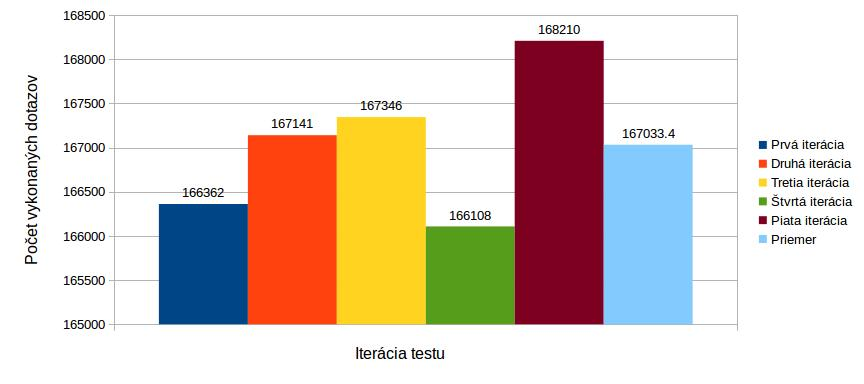
\includegraphics[width=0.9\textwidth]{faban1.jpg}
  \caption{Celkový počet vykonaných požiadaviek}
\end{figure}

\begin{figure}[H]
  \centering
      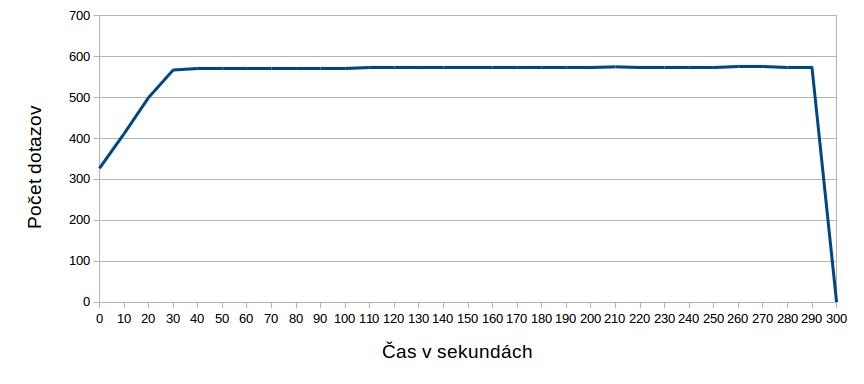
\includegraphics[width=0.9\textwidth]{faban1_distr.jpg}
  \caption{Časový priebeh vykonaných požiadaviek - aritmetický priemer všetkých iterácií}
\end{figure}

\item Gatling

Podobne ako v prípade Fabanu všetkých päť iterácií prvého testu prebehlo bez problémov. Gatling vykonal viac požiadaviek, ako Faban. Negatívom je horšia spoľahlivosť výsledkov, keď medzi najlepším a najhorším výsledkom je rozdiel 14870 vykonaných požiadaviek. Gatling má slabší štart testu v porovnaní s Fabanom, keď sa na svoje maximum dostal až 50 sekúnd po štarte, čo je pri 300 sekundovom teste veľmi dlhá doba štartu.

\begin{itemize}

\item[\textbf{1. iterácia}]\ \\
Celkový počet vykonaných požiadaviek: 302827\\
Priemerný počet vykonaných požiadaviek za sekundu: 1009,423

\item[\textbf{2. iterácia}]\ \\
Celkový počet vykonaných požiadaviek: 296602\\
Priemerný počet vykonaných požiadaviek za sekundu: 988,673

\item[\textbf{3. iterácia}]\ \\
Celkový počet vykonaných požiadaviek: 311472\\
Priemerný počet vykonaných požiadaviek za sekundu: 1038,24

\item[\textbf{4. iterácia}]\ \\
Celkový počet vykonaných požiadaviek: 303419\\
Priemerný počet vykonaných požiadaviek za sekundu: 1011,397

\item[\textbf{5. iterácia}]\ \\
Celkový počet vykonaných požiadaviek: 307912\\
Priemerný počet vykonaných požiadaviek za sekundu: 1026,373

\item[\textbf{Priemer}]\ \\
Celkový počet vykonaných požiadaviek: 304446,4\\
Priemerný počet vykonaných požiadaviek za sekundu: 1014,821

\end{itemize}

\begin{figure}[H]
  \centering
      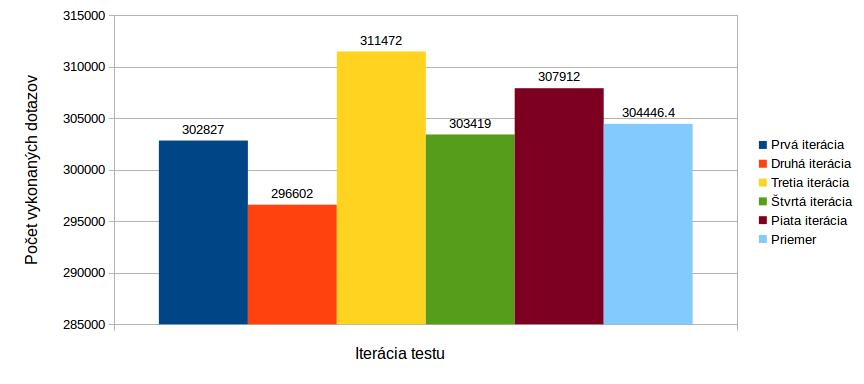
\includegraphics[width=0.9\textwidth]{gatling1.jpg}
  \caption{Celkový počet vykonaných požiadaviek}
\end{figure}

\begin{figure}[H]
  \centering
      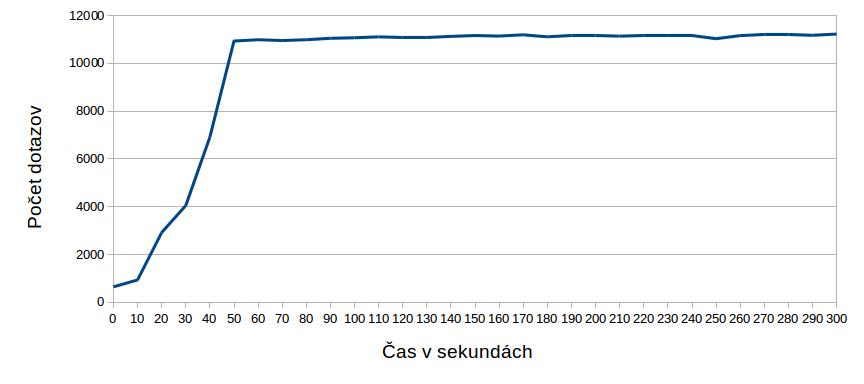
\includegraphics[width=0.9\textwidth]{gatling1_distr.jpg}
  \caption{Časový priebeh vykonaných požiadaviek - aritmetický priemer všetkých iterácií}
\end{figure}

\item Perfcake

\end{itemize}

\subsection{Testy s rastúcim počtom klientov}

\begin{itemize}

\item Apache JMeter

\item Faban

\textbf{Prvý test - 10 klientov}
\begin{itemize}

\item[\textbf{1. iterácia}]\ \\
Celkový počet vykonaných požiadaviek: 1608896\\
Priemerný počet vykonaných požiadaviek za sekundu: 5362,987

\item[\textbf{2. iterácia}]\ \\
Celkový počet vykonaných požiadaviek: 1614361\\
Priemerný počet vykonaných požiadaviek za sekundu: 5381,203

\item[\textbf{3. iterácia}]\ \\
Celkový počet vykonaných požiadaviek: 1614381\\
Priemerný počet vykonaných požiadaviek za sekundu: 5381,270

\item[\textbf{4. iterácia}]\ \\
Celkový počet vykonaných požiadaviek: 1616067\\
Priemerný počet vykonaných požiadaviek za sekundu: 5386,890

\item[\textbf{5. iterácia}]\ \\
Celkový počet vykonaných požiadaviek: 1612970\\
Priemerný počet vykonaných požiadaviek za sekundu: 5376,567

\item[\textbf{Priemer}]\ \\
Celkový počet vykonaných požiadaviek: 1613335\\
Priemerný počet vykonaných požiadaviek za sekundu: 5377,783

\end{itemize}

\begin{figure}[H]
  \centering
      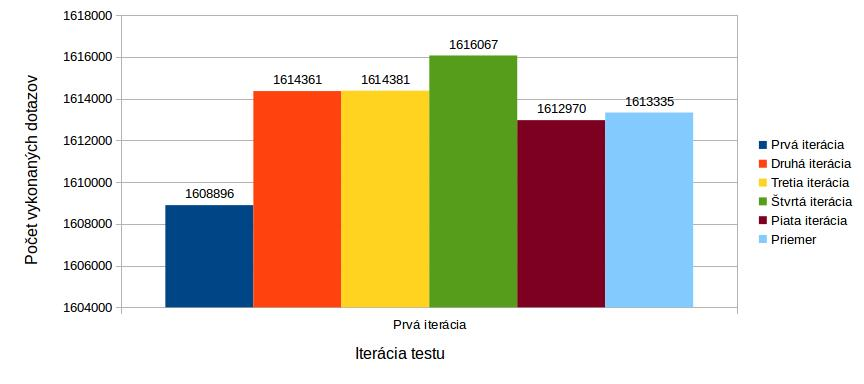
\includegraphics[width=0.9\textwidth]{faban2_1.jpg}
  \caption{Celkový počet vykonaných požiadaviek}
\end{figure}

\begin{figure}[H]
  \centering
      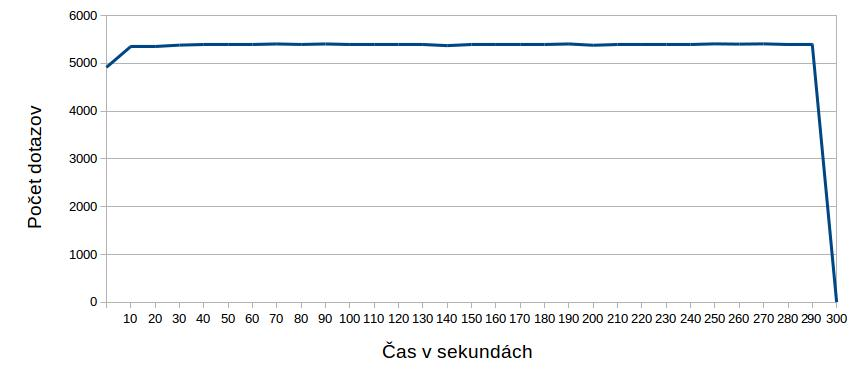
\includegraphics[width=0.9\textwidth]{faban2_1_distr.jpg}
  \caption{Časový priebeh vykonaných požiadaviek - aritmetický priemer všetkých iterácií}
\end{figure}

\textbf{Druhý test - 50 klientov}
\begin{itemize}

\item[\textbf{1. iterácia}]\ \\
Celkový počet vykonaných požiadaviek: 3300257\\
Priemerný počet vykonaných požiadaviek za sekundu: 11000,857

\item[\textbf{2. iterácia}]\ \\
Celkový počet vykonaných požiadaviek: 3304396\\
Priemerný počet vykonaných požiadaviek za sekundu: 11014,653

\item[\textbf{3. iterácia}]\ \\
Celkový počet vykonaných požiadaviek: 3286365\\
Priemerný počet vykonaných požiadaviek za sekundu: 10954,550

\item[\textbf{4. iterácia}]\ \\
Celkový počet vykonaných požiadaviek: 3280246\\
Priemerný počet vykonaných požiadaviek za sekundu: 10934,153

\item[\textbf{5. iterácia}]\ \\
Celkový počet vykonaných požiadaviek: 3303527\\
Priemerný počet vykonaných požiadaviek za sekundu: 11011,757

\item[\textbf{Priemer}]\ \\
Celkový počet vykonaných požiadaviek: 3294958,2\\
Priemerný počet vykonaných požiadaviek za sekundu: 10983,194

\end{itemize}

\begin{figure}[H]
  \centering
      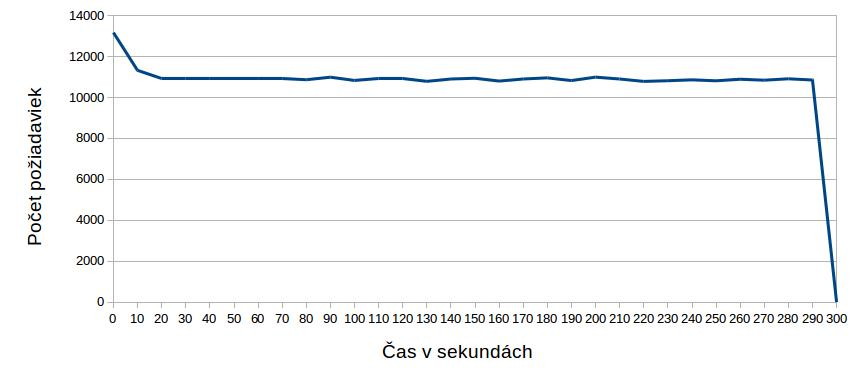
\includegraphics[width=0.9\textwidth]{faban2_2.jpg}
  \caption{Celkový počet vykonaných požiadaviek}
\end{figure}

\begin{figure}[H]
  \centering
      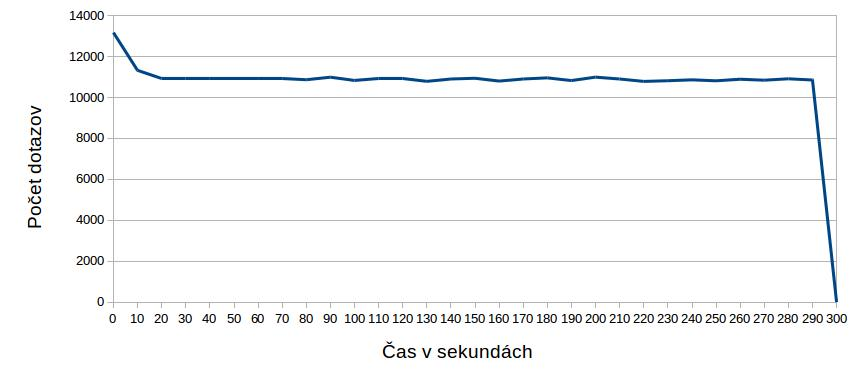
\includegraphics[width=0.9\textwidth]{faban2_2_distr.jpg}
  \caption{Časový priebeh vykonaných požiadaviek - aritmetický priemer všetkých iterácií}
\end{figure}

\textbf{Tretí test - 100 klientov}
\begin{itemize}

\item[\textbf{1. iterácia}]\ \\
Celkový počet vykonaných požiadaviek: 3208731\\
Priemerný počet vykonaných požiadaviek za sekundu: 10695,770

\item[\textbf{2. iterácia}]\ \\
Celkový počet vykonaných požiadaviek: 3232719\\
Priemerný počet vykonaných požiadaviek za sekundu: 10775,730

\item[\textbf{3. iterácia}]\ \\
Celkový počet vykonaných požiadaviek: 3220658\\
Priemerný počet vykonaných požiadaviek za sekundu: 10735,527

\item[\textbf{4. iterácia}]\ \\
Celkový počet vykonaných požiadaviek: 3225564\\
Priemerný počet vykonaných požiadaviek za sekundu: 10751,880

\item[\textbf{5. iterácia}]\ \\
Test zlyhal, objavila sa chyba: Error initializing driver object. com.sun.fa-ban.driver.ConfigurationException: Only single host:port currently supported.\\ Chyba sa vyskytla len pri jednej iterácii a týka sa inicializácie testu Fabanom.\hypertarget{label}{}

\item[\textbf{Priemer}]\ \\
Celkový počet vykonaných požiadaviek: 3221918\\
Priemerný počet vykonaných požiadaviek za sekundu: 10739,727

\end{itemize}

\begin{figure}[H]
  \centering
      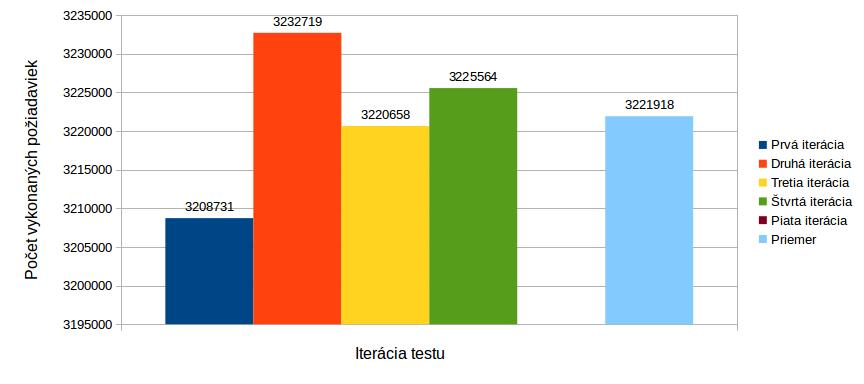
\includegraphics[width=0.9\textwidth]{faban2_3.jpg}
  \caption{Celkový počet vykonaných požiadaviek}
\end{figure}

\begin{figure}[H]
  \centering
      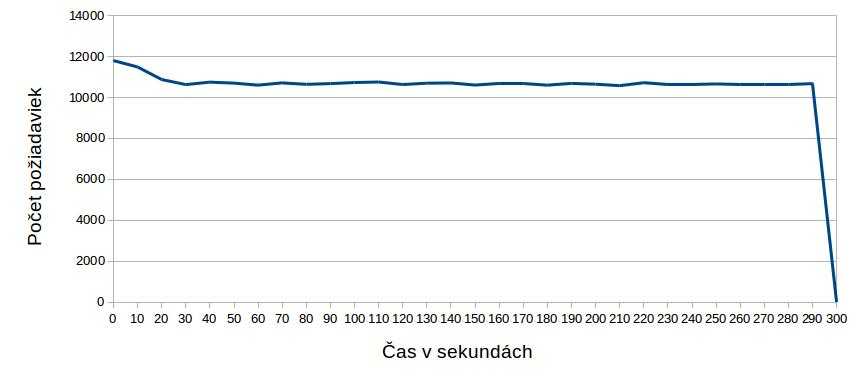
\includegraphics[width=0.9\textwidth]{faban2_3_distr.jpg}
  \caption{Časový priebeh vykonaných požiadaviek - aritmetický priemer všetkých iterácií}
\end{figure}

\textbf{Štvrtý test - 150 klientov}
\begin{itemize}

\item[\textbf{1. iterácia}]\ \\
Celkový počet vykonaných požiadaviek: 3189387\\
Priemerný počet vykonaných požiadaviek za sekundu: 10631,290

\item[\textbf{2. iterácia}]\ \\
Celkový počet vykonaných požiadaviek: 3186480\\
Priemerný počet vykonaných požiadaviek za sekundu: 10621,600

\item[\textbf{3. iterácia}]\ \\
Celkový počet vykonaných požiadaviek: 3184917\\
Priemerný počet vykonaných požiadaviek za sekundu: 10616,390

\item[\textbf{4. iterácia}]\ \\
Celkový počet vykonaných požiadaviek: 3187227\\
Priemerný počet vykonaných požiadaviek za sekundu: 10624,090

\item[\textbf{5. iterácia}]\ \\
Celkový počet vykonaných požiadaviek: 3192963\\
Priemerný počet vykonaných požiadaviek za sekundu: 10643,210

\item[\textbf{Priemer}]\ \\
Celkový počet vykonaných požiadaviek: 3188194,8\\
Priemerný počet vykonaných požiadaviek za sekundu: 10627,316

\end{itemize}

\begin{figure}[H]
  \centering
      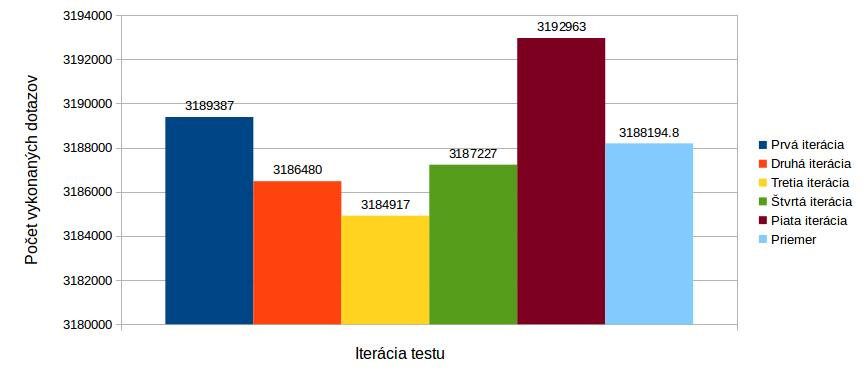
\includegraphics[width=0.9\textwidth]{faban2_4.jpg}
  \caption{Celkový počet vykonaných požiadaviek}
\end{figure}

\begin{figure}[H]
  \centering
      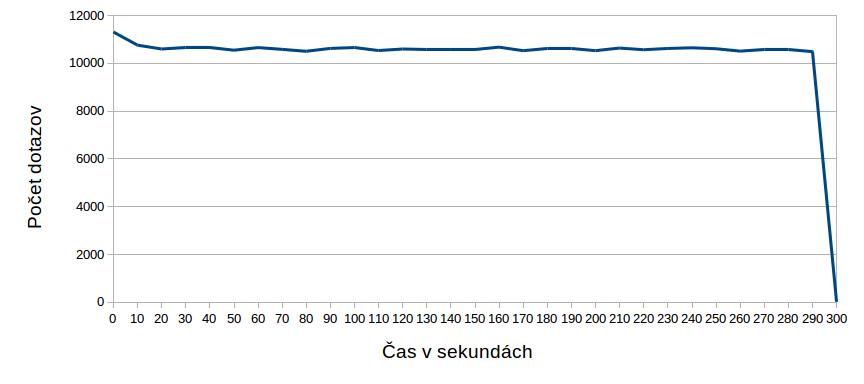
\includegraphics[width=0.9\textwidth]{faban2_4_distr.jpg}
  \caption{Časový priebeh vykonaných požiadaviek - aritmetický priemer všetkých iterácií}
\end{figure}

\textbf{Piaty test - 200 klientov}
\begin{itemize}

\item[\textbf{1. iterácia}]\ \\
Celkový počet vykonaných požiadaviek: 3186355\\
Priemerný počet vykonaných požiadaviek za sekundu: 10621,183

\item[\textbf{2. iterácia}]\ \\
Celkový počet vykonaných požiadaviek: 3206037\\
Priemerný počet vykonaných požiadaviek za sekundu: 10686,790

\item[\textbf{3. iterácia}]\ \\
Rovnaká chyba ako v \hyperlink{label}{piatej iterácii tretieho testu}.

\item[\textbf{4. iterácia}]\ \\
Celkový počet vykonaných požiadaviek: 3187980\\
Priemerný počet vykonaných požiadaviek za sekundu: 10626,600

\item[\textbf{5. iterácia}]\ \\
Celkový počet vykonaných požiadaviek: 3217781\\
Priemerný počet vykonaných požiadaviek za sekundu: 10725,937

\item[\textbf{Priemer}]\ \\
Celkový počet vykonaných požiadaviek: 3199538,25\\
Priemerný počet vykonaných požiadaviek za sekundu: 10665,128

\end{itemize}

\begin{figure}[H]
  \centering
      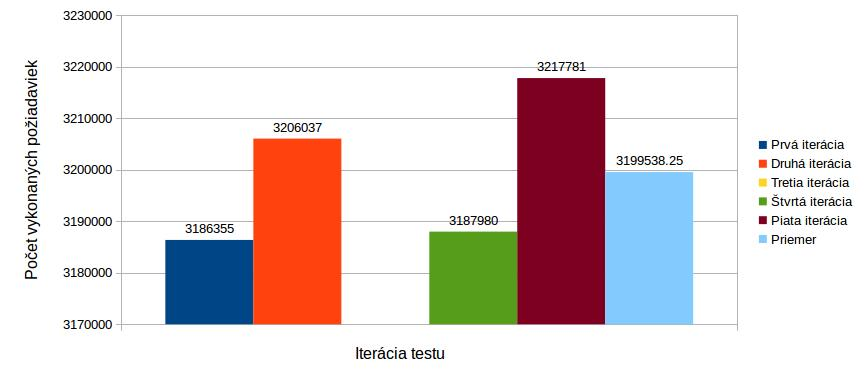
\includegraphics[width=0.9\textwidth]{faban2_5.jpg}
  \caption{Celkový počet vykonaných požiadaviek}
\end{figure}

\begin{figure}[H]
  \centering
      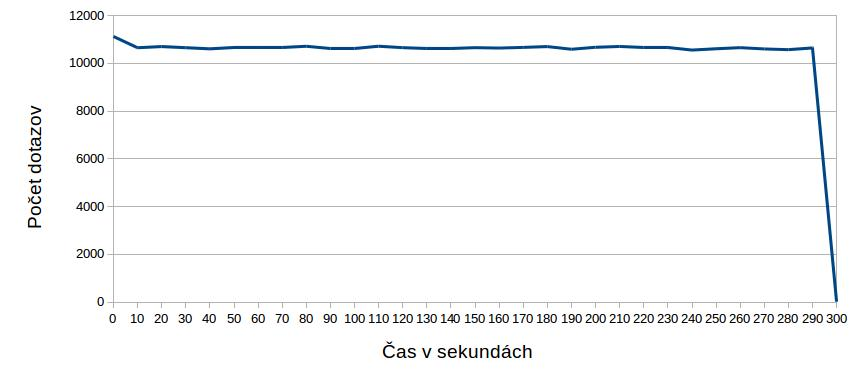
\includegraphics[width=0.9\textwidth]{faban2_5_distr.jpg}
  \caption{Časový priebeh vykonaných požiadaviek - aritmetický priemer všetkých iterácií}
\end{figure}

Z výsledkov testu je jasne vidieť, že Faban dosiahol najvyšší výkon počas testu s 50 klientmi. Testy so 100, 150 a 200 klientmi majú slabšie výsledky. Ako veľké negatívum hodnotím zlyhanie poslednej iterácie testu so 100 klientmi a zlyhanie 3. iterácie testu s 200 klientmi. Chybu som spozoroval už pri spúšťaní testov na nečisto. Vyskytuje sa úplne náhodne a nepodarilo sa mi zistiť, prečo k nej dochádza.
\par Na druhej strane oproti základnému testu s jedným klientom klesol čas potrebný k dosiahnutiu maximálneho výkonu. V teste s 10 klientmi Faban potreboval len 10 sekúnd na dosiahnutie maximálneho výkonu, pričom rozdiel v počte požiadaviek tvoril len 8\%, kdežto v základnom teste to bolo až 20\%. Zvyšné modifikácie dokonca zaznamenali najvyšší výkon hneď pri štarte.



\item Gatling

\textbf{Prvý test - 10 klientov}
\begin{itemize}

\item[\textbf{1. iterácia}]\ \\
Celkový počet vykonaných požiadaviek: 1831121\\
Priemerný počet vykonaných požiadaviek za sekundu: 6103,737

\item[\textbf{2. iterácia}]\ \\
Celkový počet vykonaných požiadaviek: 1818769\\
Priemerný počet vykonaných požiadaviek za sekundu: 6062,563

\item[\textbf{3. iterácia}]\ \\
Celkový počet vykonaných požiadaviek: 1835757\\
Priemerný počet vykonaných požiadaviek za sekundu: 6119,190

\item[\textbf{4. iterácia}]\ \\
Celkový počet vykonaných požiadaviek: 1812333\\
Priemerný počet vykonaných požiadaviek za sekundu: 6041,110

\item[\textbf{5. iterácia}]\ \\
Celkový počet vykonaných požiadaviek: 1827221\\
Priemerný počet vykonaných požiadaviek za sekundu: 6090,737

\item[\textbf{Priemer}]\ \\
Celkový počet vykonaných požiadaviek: 1822361\\
Priemerný počet vykonaných požiadaviek za sekundu: 6074,537

\end{itemize}

\begin{figure}[H]
  \centering
      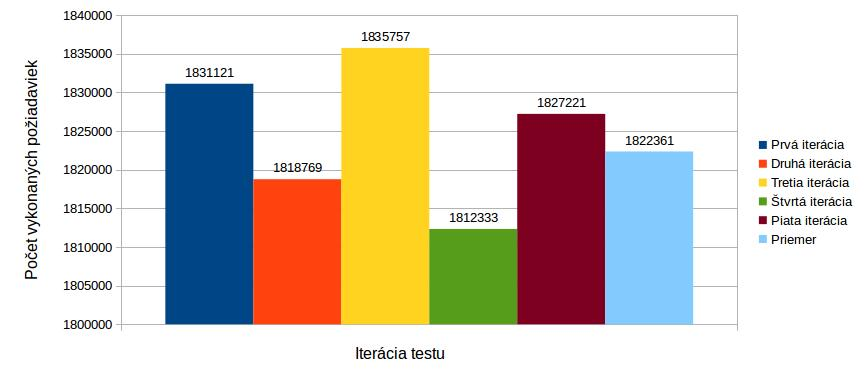
\includegraphics[width=0.9\textwidth]{gatling2_1.jpg}
  \caption{Celkový počet vykonaných požiadaviek}
\end{figure}

\begin{figure}[H]
  \centering
      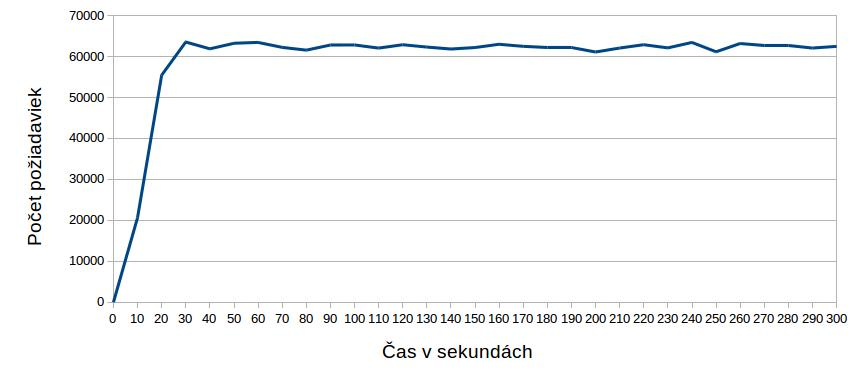
\includegraphics[width=0.9\textwidth]{gatling2_1_distr.jpg}
  \caption{Časový priebeh vykonaných požiadaviek - aritmetický priemer všetkých iterácií}
\end{figure}

\textbf{Druhý test - 50 klientov}
\begin{itemize}

\item[\textbf{1. iterácia}]\ \\
Celkový počet vykonaných požiadaviek: 1918599\\
Priemerný počet vykonaných požiadaviek za sekundu: 6395,330

\item[\textbf{2. iterácia}]\ \\
Celkový počet vykonaných požiadaviek: 1952562\\
Priemerný počet vykonaných požiadaviek za sekundu: 6508,540

\item[\textbf{3. iterácia}]\ \\
Celkový počet vykonaných požiadaviek: 1913446\\
Priemerný počet vykonaných požiadaviek za sekundu: 6378,153

\item[\textbf{4. iterácia}]\ \\
Celkový počet vykonaných požiadaviek: 1935923\\
Priemerný počet vykonaných požiadaviek za sekundu: 6453,077

\item[\textbf{5. iterácia}]\ \\
Celkový počet vykonaných požiadaviek: 1905032\\
Priemerný počet vykonaných požiadaviek za sekundu: 6350,107

\item[\textbf{Priemer}]\ \\
Celkový počet vykonaných požiadaviek: 1928029\\
Priemerný počet vykonaných požiadaviek za sekundu: 6426,763

\end{itemize}

\begin{figure}[H]
  \centering
      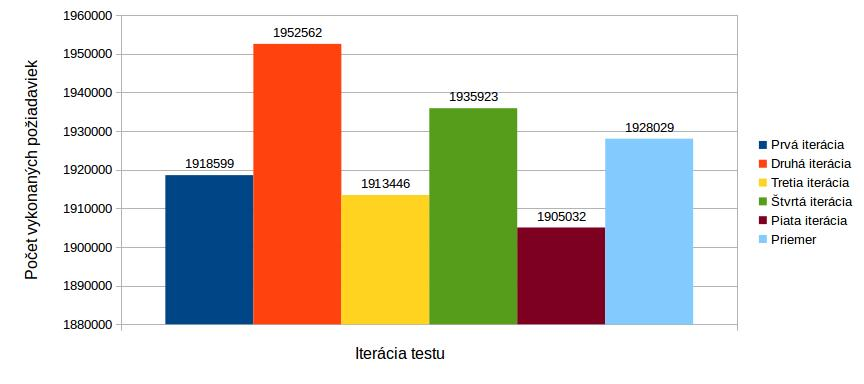
\includegraphics[width=0.9\textwidth]{gatling2_2.jpg}
  \caption{Celkový počet vykonaných požiadaviek}
\end{figure}

\begin{figure}[H]
  \centering
      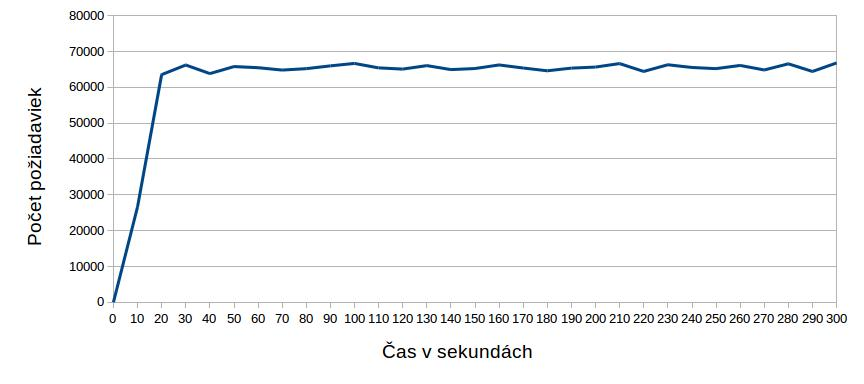
\includegraphics[width=0.9\textwidth]{gatling2_2_distr.jpg}
  \caption{Časový priebeh vykonaných požiadaviek - aritmetický priemer všetkých iterácií}
\end{figure}

\textbf{Tretí test - 100 klientov}
\begin{itemize}

\item[\textbf{1. iterácia}]\ \\
Celkový počet vykonaných požiadaviek: 2136292\\
Priemerný počet vykonaných požiadaviek za sekundu: 7120,973

\item[\textbf{2. iterácia}]\ \\
Celkový počet vykonaných požiadaviek: 2167595\\
Priemerný počet vykonaných požiadaviek za sekundu: 7225,317

\item[\textbf{3. iterácia}]\ \\
Celkový počet vykonaných požiadaviek: 2128423\\
Priemerný počet vykonaných požiadaviek za sekundu: 7094,743

\item[\textbf{4. iterácia}]\ \\
Celkový počet vykonaných požiadaviek: 2108157\\
Priemerný počet vykonaných požiadaviek za sekundu: 7027,190

\item[\textbf{5. iterácia}]\ \\
Celkový počet vykonaných požiadaviek: 2148207\\
Priemerný počet vykonaných požiadaviek za sekundu: 7160,690

\item[\textbf{Priemer}]\ \\
Celkový počet vykonaných požiadaviek: 2140062,75\\
Priemerný počet vykonaných požiadaviek za sekundu: 7133,543

\end{itemize}

\begin{figure}[H]
  \centering
      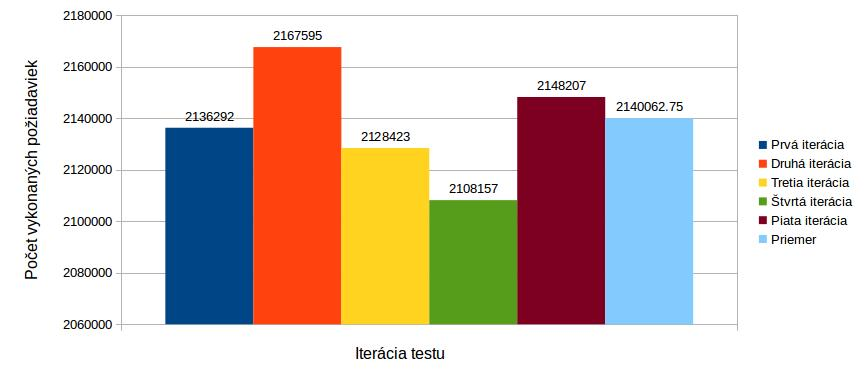
\includegraphics[width=0.9\textwidth]{gatling2_3.jpg}
  \caption{Celkový počet vykonaných požiadaviek}
\end{figure}

\begin{figure}[H]
  \centering
      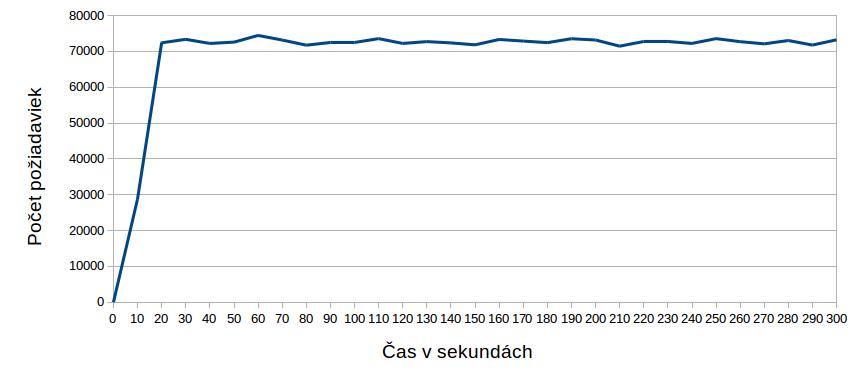
\includegraphics[width=0.9\textwidth]{gatling2_3_distr.jpg}
  \caption{Časový priebeh vykonaných požiadaviek - aritmetický priemer všetkých iterácií}
\end{figure}

\textbf{Štvrtý test - 150 klientov}
\begin{itemize}

\item[\textbf{1. iterácia}]\ \\
Celkový počet vykonaných požiadaviek: 2323968\\
Priemerný počet vykonaných požiadaviek za sekundu: 7746,560

\item[\textbf{2. iterácia}]\ \\
Celkový počet vykonaných požiadaviek: 2322686\\
Priemerný počet vykonaných požiadaviek za sekundu: 7742,287

\item[\textbf{3. iterácia}]\ \\
Celkový počet vykonaných požiadaviek: 2336059\\
Priemerný počet vykonaných požiadaviek za sekundu: 7786,863

\item[\textbf{4. iterácia}]\ \\
Celkový počet vykonaných požiadaviek: 2334234\\
Priemerný počet vykonaných požiadaviek za sekundu: 7780,780

\item[\textbf{5. iterácia}]\ \\
Celkový počet vykonaných požiadaviek: 2352479\\
Priemerný počet vykonaných požiadaviek za sekundu: 7841,597

\item[\textbf{Priemer}]\ \\
Celkový počet vykonaných požiadaviek: 2333341,75\\
Priemerný počet vykonaných požiadaviek za sekundu: 7777,806

\end{itemize}

\begin{figure}[H]
  \centering
      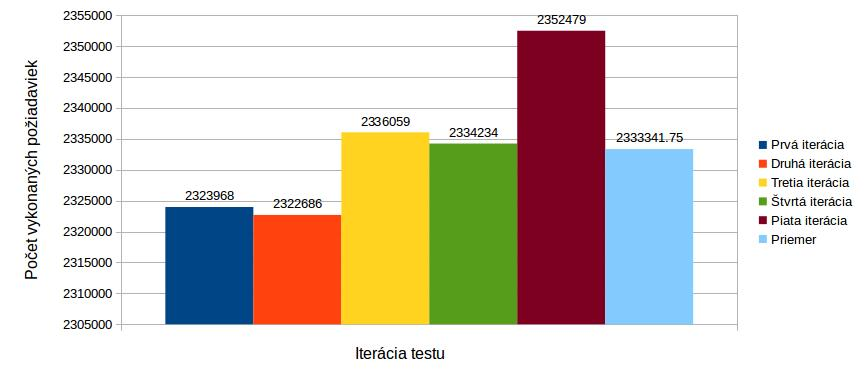
\includegraphics[width=0.9\textwidth]{gatling2_4.jpg}
  \caption{Celkový počet vykonaných požiadaviek}
\end{figure}

\begin{figure}[H]
  \centering
      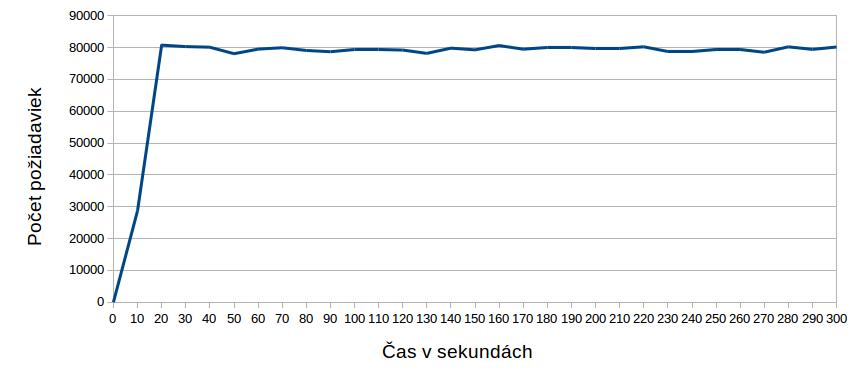
\includegraphics[width=0.9\textwidth]{gatling2_4_distr.jpg}
  \caption{Časový priebeh vykonaných požiadaviek - aritmetický priemer všetkých iterácií}
\end{figure}

\textbf{Piaty test - 200 klientov}
\begin{itemize}

\item[\textbf{1. iterácia}]\ \\
Celkový počet vykonaných požiadaviek: 2508025\\
Priemerný počet vykonaných požiadaviek za sekundu: 8360,083

\item[\textbf{2. iterácia}]\ \\
Celkový počet vykonaných požiadaviek: 2511472\\
Priemerný počet vykonaných požiadaviek za sekundu: 8371,573

\item[\textbf{3. iterácia}]\ \\
Celkový počet vykonaných požiadaviek: 2490477\\
Priemerný počet vykonaných požiadaviek za sekundu: 8301,590

\item[\textbf{4. iterácia}]\ \\
Celkový počet vykonaných požiadaviek: 2536607\\
Priemerný počet vykonaných požiadaviek za sekundu: 8455,357

\item[\textbf{5. iterácia}]\ \\
Celkový počet vykonaných požiadaviek: 2550135\\
Priemerný počet vykonaných požiadaviek za sekundu: 8500,450

\item[\textbf{Priemer}]\ \\
Celkový počet vykonaných požiadaviek: 2526559,75\\
Priemerný počet vykonaných požiadaviek za sekundu: 8421,866

\end{itemize}

\begin{figure}[H]
  \centering
      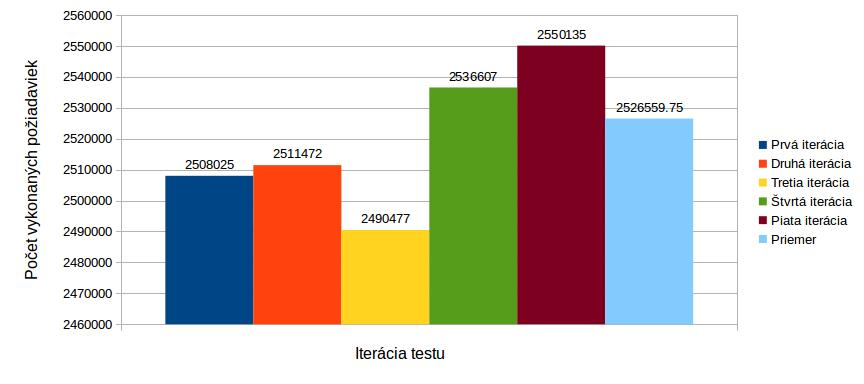
\includegraphics[width=0.9\textwidth]{gatling2_5.jpg}
  \caption{Celkový počet vykonaných požiadaviek}
\end{figure}

\begin{figure}[H]
  \centering
      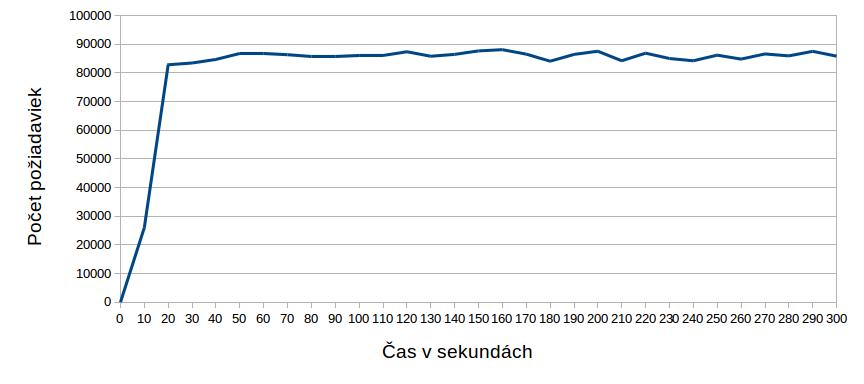
\includegraphics[width=0.9\textwidth]{gatling2_5_distr.jpg}
  \caption{Časový priebeh vykonaných požiadaviek - aritmetický priemer všetkých iterácií}
\end{figure}

\item Perfcake

\end{itemize}

\subsection{Testy s rastúcou veľkosťou správ}

\begin{itemize}

\item Apache JMeter

\item Faban

\textbf{Prvý test - 5 znaková správa}
\begin{itemize}

\item[\textbf{1. iterácia}]\ \\
Celkový počet vykonaných požiadaviek: 6807453\\
Priemerný počet vykonaných požiadaviek za sekundu: 22691,510

\item[\textbf{2. iterácia}]\ \\
Celkový počet vykonaných požiadaviek: 6802899\\
Priemerný počet vykonaných požiadaviek za sekundu: 22676,330

\item[\textbf{3. iterácia}]\ \\
Celkový počet vykonaných požiadaviek: 6857271\\
Priemerný počet vykonaných požiadaviek za sekundu: 22857,570

\item[\textbf{4. iterácia}]\ \\
Celkový počet vykonaných požiadaviek: 6831598\\
Priemerný počet vykonaných požiadaviek za sekundu: 22771,993

\item[\textbf{5. iterácia}]\ \\
Celkový počet vykonaných požiadaviek: 6837934\\
Priemerný počet vykonaných požiadaviek za sekundu: 22793,113

\item[\textbf{Priemer}]\ \\
Celkový počet vykonaných požiadaviek: 6827431\\
Priemerný počet vykonaných požiadaviek za sekundu: 22758,103

\end{itemize}

\begin{figure}[H]
  \centering
      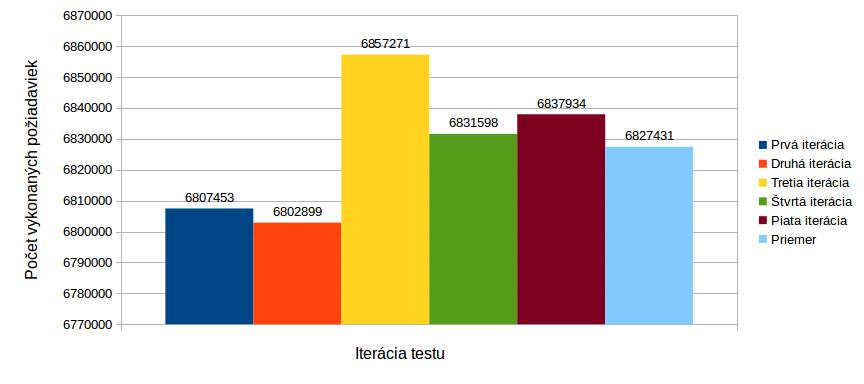
\includegraphics[width=0.9\textwidth]{faban3_1.jpg}
  \caption{Celkový počet vykonaných požiadaviek}
\end{figure}

\begin{figure}[H]
  \centering
      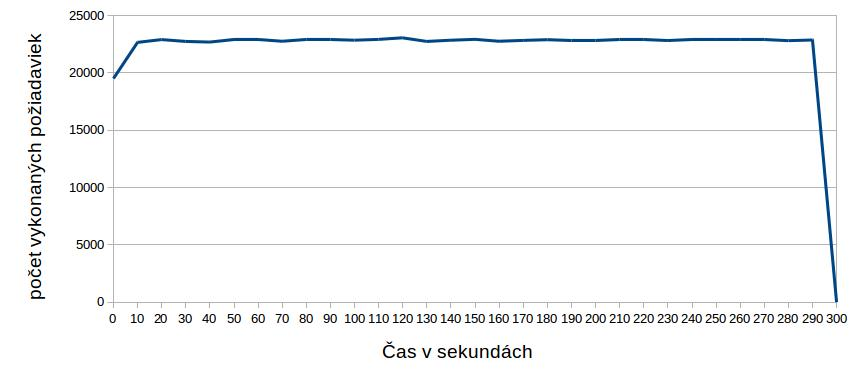
\includegraphics[width=0.9\textwidth]{faban3_1_distr.jpg}
  \caption{Časový priebeh vykonaných požiadaviek - aritmetický priemer všetkých iterácií}
\end{figure}

\textbf{Druhý test - 1024 znaková správa (1 KB)}
\begin{itemize}

\item[\textbf{1. iterácia}]\ \\
Celkový počet vykonaných požiadaviek: 339326\\
Priemerný počet vykonaných požiadaviek za sekundu: 1131,087

\item[\textbf{2. iterácia}]\ \\
Chyba, \hyperlink{label}{viď. test 2.3.5}.

\item[\textbf{3. iterácia}]\ \\
Celkový počet vykonaných požiadaviek: 339615\\
Priemerný počet vykonaných požiadaviek za sekundu: 1132,050

\item[\textbf{4. iterácia}]\ \\
Chyba, \hyperlink{label}{viď. test 2.3.5}.

\item[\textbf{5. iterácia}]\ \\
Celkový počet vykonaných požiadaviek: 336776\\
Priemerný počet vykonaných požiadaviek za sekundu: 1122,587

\item[\textbf{Priemer}]\ \\
Celkový počet vykonaných požiadaviek: 338572,3\\
Priemerný počet vykonaných požiadaviek za sekundu: 1128,574

\end{itemize}

\begin{figure}[H]
  \centering
      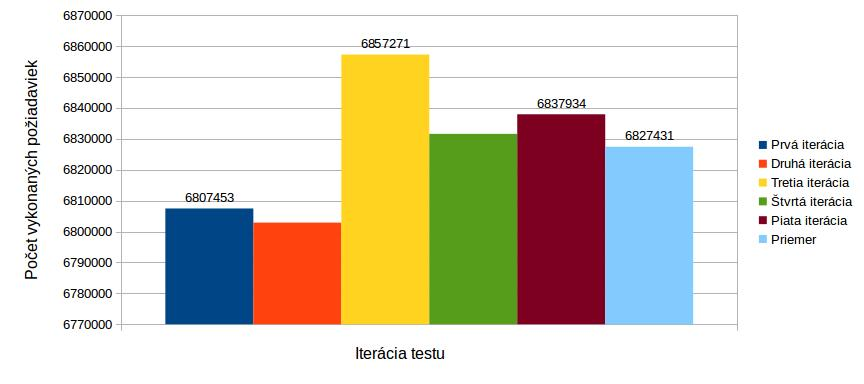
\includegraphics[width=0.9\textwidth]{faban3_2.jpg}
  \caption{Celkový počet vykonaných požiadaviek}
\end{figure}

\begin{figure}[H]
  \centering
      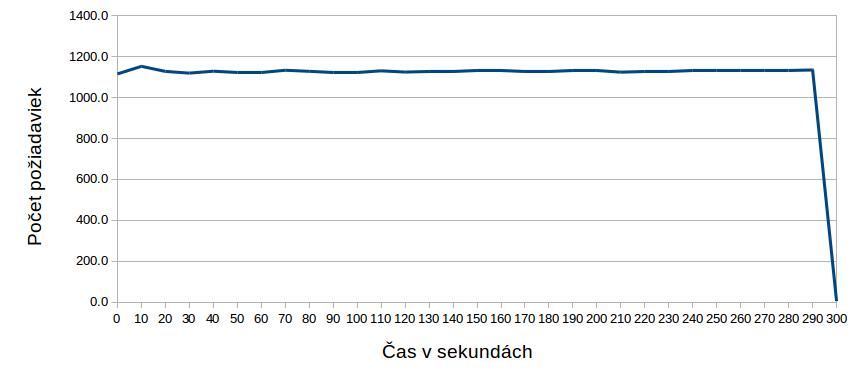
\includegraphics[width=0.9\textwidth]{faban3_2_distr.jpg}
  \caption{Časový priebeh vykonaných požiadaviek - aritmetický priemer všetkých iterácií}
\end{figure}

\textbf{Tretí test - 5120 znaková správa (5 KB)}
\begin{itemize}

\item[\textbf{1. iterácia}]\ \\
Celkový počet vykonaných požiadaviek: 68625\\
Priemerný počet vykonaných požiadaviek za sekundu: 228,750

\item[\textbf{2. iterácia}]\ \\
Chyba, \hyperlink{label}{viď. test 2.3.5}.

\item[\textbf{3. iterácia}]\ \\
Celkový počet vykonaných požiadaviek: 68748\\
Priemerný počet vykonaných požiadaviek za sekundu: 229,160

\item[\textbf{4. iterácia}]\ \\
Chyba, \hyperlink{label}{viď. test 2.3.5}.

\item[\textbf{5. iterácia}]\ \\
Celkový počet vykonaných požiadaviek: 68932\\
Priemerný počet vykonaných požiadaviek za sekundu: 229,773

\item[\textbf{Priemer}]\ \\
Celkový počet vykonaných požiadaviek: 68768,3\\
Priemerný počet vykonaných požiadaviek za sekundu: 229,228

\end{itemize}

\begin{figure}[H]
  \centering
      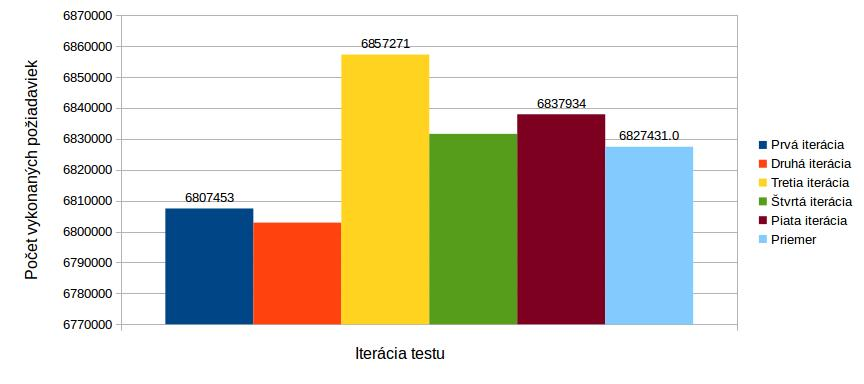
\includegraphics[width=0.9\textwidth]{faban3_3.jpg}
  \caption{Celkový počet vykonaných požiadaviek}
\end{figure}

\begin{figure}[H]
  \centering
      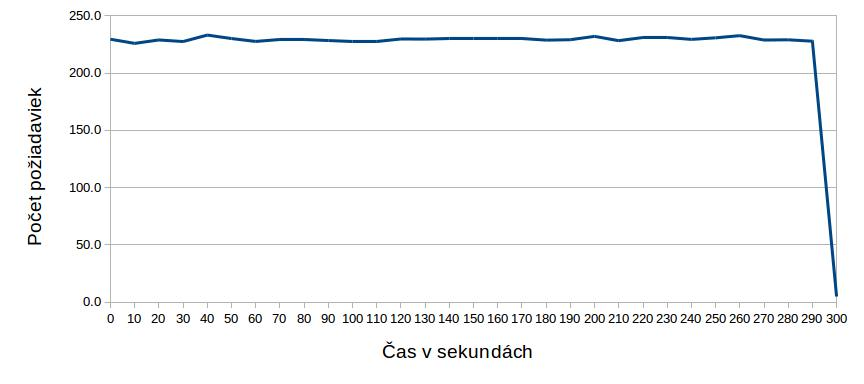
\includegraphics[width=0.9\textwidth]{faban3_3_distr.jpg}
  \caption{Časový priebeh vykonaných požiadaviek - aritmetický priemer všetkých iterácií}
\end{figure}

\textbf{Štvrtý test - 51200 znaková správa (50 KB)}
\begin{itemize}

\item[\textbf{1. iterácia}]\ \\
Celkový počet vykonaných požiadaviek: 6794\\
Priemerný počet vykonaných požiadaviek za sekundu: 22,647

\item[\textbf{2. iterácia}]\ \\
Celkový počet vykonaných požiadaviek: 6743\\
Priemerný počet vykonaných požiadaviek za sekundu: 22,477

\item[\textbf{3. iterácia}]\ \\
Celkový počet vykonaných požiadaviek: 6752\\
Priemerný počet vykonaných požiadaviek za sekundu: 22,507

\item[\textbf{4. iterácia}]\ \\
Chyba, \hyperlink{label}{viď. test 2.3.5}.

\item[\textbf{5. iterácia}]\ \\
Celkový počet vykonaných požiadaviek: 6772\\
Priemerný počet vykonaných požiadaviek za sekundu: 22,573

\item[\textbf{Priemer}]\ \\
Celkový počet vykonaných požiadaviek: 6765,3\\
Priemerný počet vykonaných požiadaviek za sekundu: 22,551

\end{itemize}

\begin{figure}[H]
  \centering
      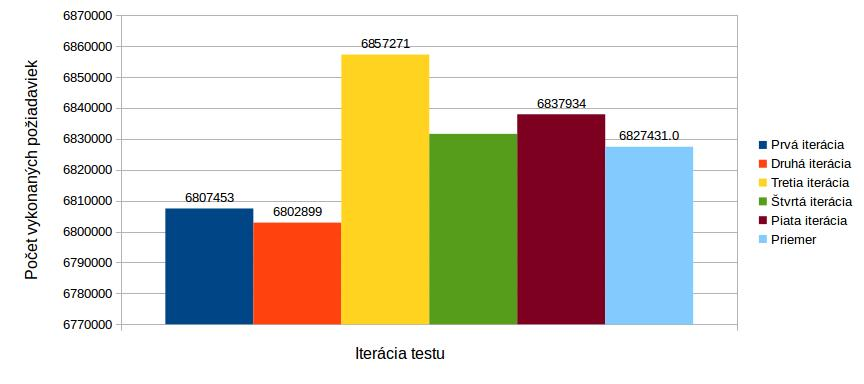
\includegraphics[width=0.9\textwidth]{faban3_4.jpg}
  \caption{Celkový počet vykonaných požiadaviek}
\end{figure}

\begin{figure}[H]
  \centering
      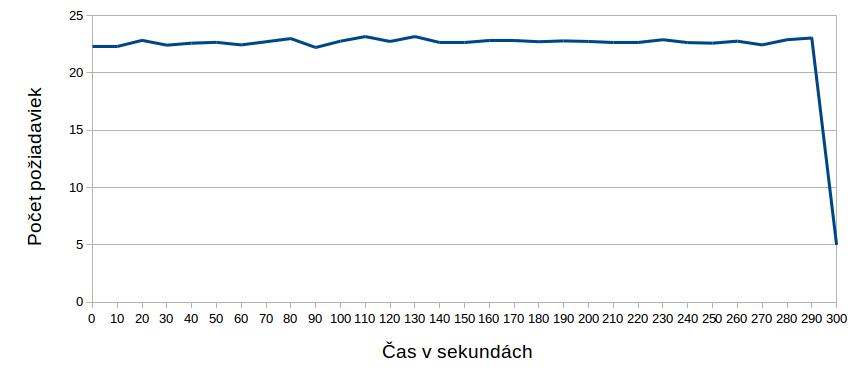
\includegraphics[width=0.9\textwidth]{faban3_4_distr.jpg}
  \caption{Časový priebeh vykonaných požiadaviek - aritmetický priemer všetkých iterácií}
\end{figure}

\textbf{Piaty test - 512000 znaková správa (500 KB)}
\begin{itemize}

\item[\textbf{1. iterácia}]\ \\
Chyba, \hyperlink{label}{viď. test 2.3.5}.

\item[\textbf{2. iterácia}]\ \\
Celkový počet vykonaných požiadaviek: 610\\
Priemerný počet vykonaných požiadaviek za sekundu: 2,033

\item[\textbf{3. iterácia}]\ \\
Celkový počet vykonaných požiadaviek: 612\\
Priemerný počet vykonaných požiadaviek za sekundu: 2,040

\item[\textbf{4. iterácia}]\ \\
Celkový počet vykonaných požiadaviek: 613\\
Priemerný počet vykonaných požiadaviek za sekundu: 2,043

\item[\textbf{5. iterácia}]\ \\
Celkový počet vykonaných požiadaviek: 615\\
Priemerný počet vykonaných požiadaviek za sekundu: 2,050

\item[\textbf{Priemer}]\ \\
Celkový počet vykonaných požiadaviek: 612,5\\
Priemerný počet vykonaných požiadaviek za sekundu: 2,042

\end{itemize}

\begin{figure}[H]
  \centering
      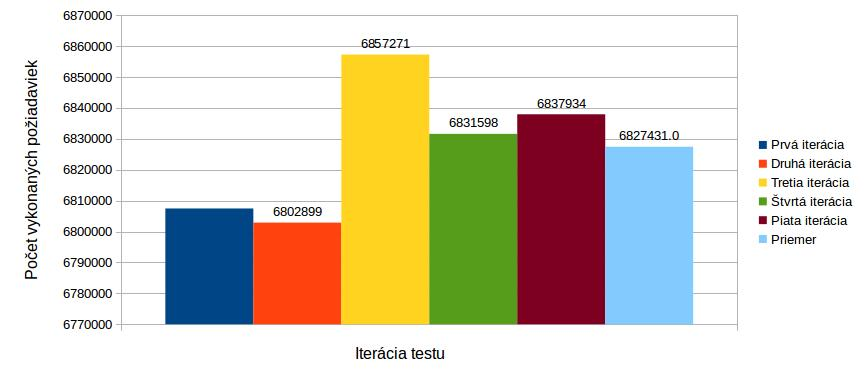
\includegraphics[width=0.9\textwidth]{faban3_5.jpg}
  \caption{Celkový počet vykonaných požiadaviek}
\end{figure}

\begin{figure}[H]
  \centering
      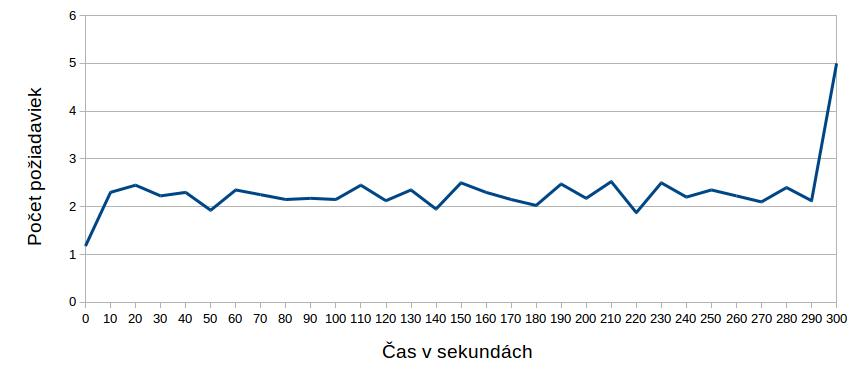
\includegraphics[width=0.9\textwidth]{faban3_5_distr.jpg}
  \caption{Časový priebeh vykonaných požiadaviek - aritmetický priemer všetkých iterácií}
\end{figure}


\item Gatling

\textbf{Prvý test - 5 znaková správa}
\begin{itemize}

\item[\textbf{1. iterácia}]\ \\
Celkový počet vykonaných požiadaviek: 2578507\\
Priemerný počet vykonaných požiadaviek za sekundu: 8595,023

\item[\textbf{2. iterácia}]\ \\
Celkový počet vykonaných požiadaviek: 2606448\\
Priemerný počet vykonaných požiadaviek za sekundu: 8688,160

\item[\textbf{3. iterácia}]\ \\
Celkový počet vykonaných požiadaviek: 2609597\\
Priemerný počet vykonaných požiadaviek za sekundu: 8698,657

\item[\textbf{4. iterácia}]\ \\
Celkový počet vykonaných požiadaviek: 2516099\\
Priemerný počet vykonaných požiadaviek za sekundu: 8386,997

\item[\textbf{5. iterácia}]\ \\
Celkový počet vykonaných požiadaviek: 2586725\\
Priemerný počet vykonaných požiadaviek za sekundu: 8622,417

\item[\textbf{Priemer}]\ \\
Celkový počet vykonaných požiadaviek: 2571944,75\\
Priemerný počet vykonaných požiadaviek za sekundu: 8573,149

\end{itemize}

\begin{figure}[H]
  \centering
      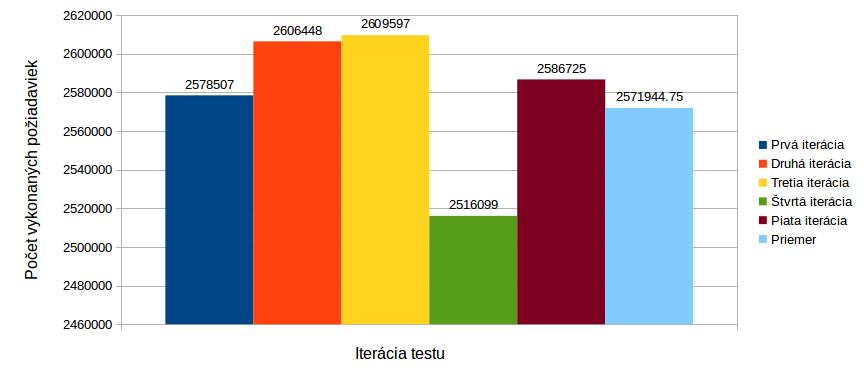
\includegraphics[width=0.9\textwidth]{gatling3_1.jpg}
  \caption{Celkový počet vykonaných požiadaviek}
\end{figure}

\begin{figure}[H]
  \centering
      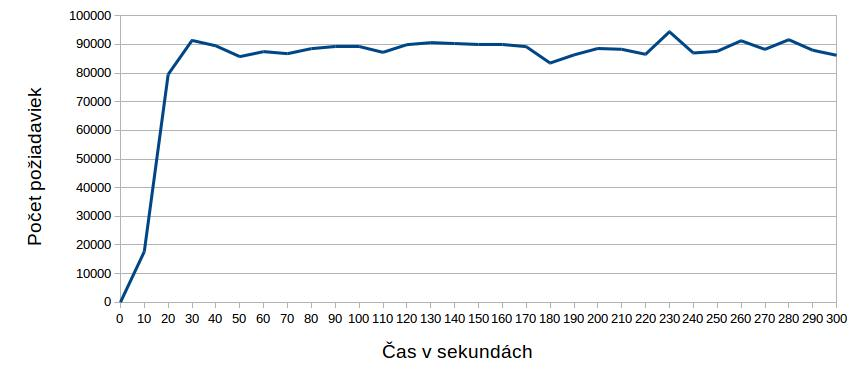
\includegraphics[width=0.9\textwidth]{gatling3_1_distr.jpg}
  \caption{Časový priebeh vykonaných požiadaviek - aritmetický priemer všetkých iterácií}
\end{figure}

\textbf{Druhý test - 1024 znaková správa (1 KB)}
\begin{itemize}

\item[\textbf{1. iterácia}]\ \\
Celkový počet vykonaných požiadaviek: 334502\\
Priemerný počet vykonaných požiadaviek za sekundu: 1115,007

\item[\textbf{2. iterácia}]\ \\
Celkový počet vykonaných požiadaviek: 337257\\
Priemerný počet vykonaných požiadaviek za sekundu: 1124,190

\item[\textbf{3. iterácia}]\ \\
Celkový počet vykonaných požiadaviek: 337315\\
Priemerný počet vykonaných požiadaviek za sekundu: 1124,383

\item[\textbf{4. iterácia}]\ \\
Celkový počet vykonaných požiadaviek: 334833\\
Priemerný počet vykonaných požiadaviek za sekundu: 1116,110

\item[\textbf{5. iterácia}]\ \\
Celkový počet vykonaných požiadaviek: 336393\\
Priemerný počet vykonaných požiadaviek za sekundu: 1121,310

\item[\textbf{Priemer}]\ \\
Celkový počet vykonaných požiadaviek: 335746,25\\
Priemerný počet vykonaných požiadaviek za sekundu: 1119,154

\end{itemize}

\begin{figure}[H]
  \centering
      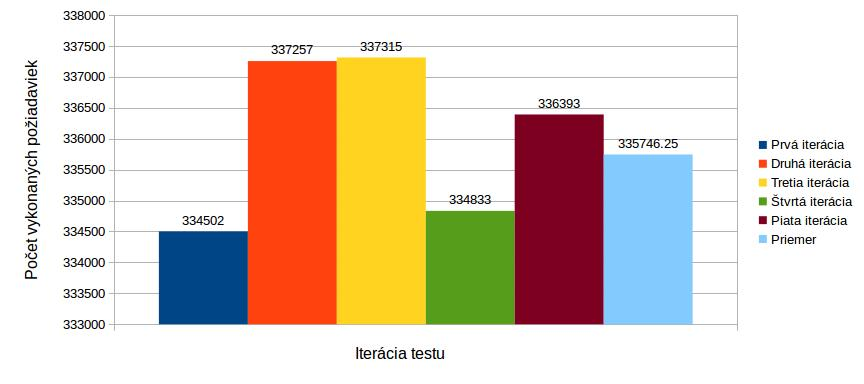
\includegraphics[width=0.9\textwidth]{gatling3_2.jpg}
  \caption{Celkový počet vykonaných požiadaviek}
\end{figure}

\begin{figure}[H]
  \centering
      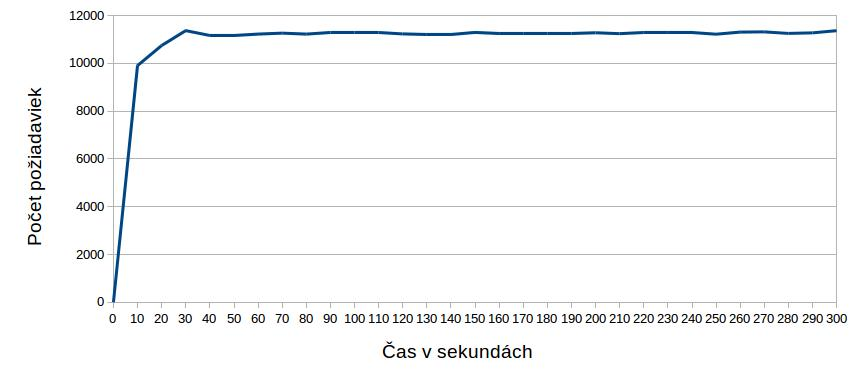
\includegraphics[width=0.9\textwidth]{gatling3_2_distr.jpg}
  \caption{Časový priebeh vykonaných požiadaviek - aritmetický priemer všetkých iterácií}
\end{figure}

\textbf{Tretí test - 5120 znaková správa (5 KB)}
\begin{itemize}

\item[\textbf{1. iterácia}]\ \\
Celkový počet vykonaných požiadaviek: 68448\\
Priemerný počet vykonaných požiadaviek za sekundu: 228,160

\item[\textbf{2. iterácia}]\ \\
Celkový počet vykonaných požiadaviek: 68762\\
Priemerný počet vykonaných požiadaviek za sekundu: 229,207

\item[\textbf{3. iterácia}]\ \\
Celkový počet vykonaných požiadaviek: 68519\\
Priemerný počet vykonaných požiadaviek za sekundu: 228,397

\item[\textbf{4. iterácia}]\ \\
Celkový počet vykonaných požiadaviek: 68745\\
Priemerný počet vykonaných požiadaviek za sekundu: 229,150

\item[\textbf{5. iterácia}]\ \\
Celkový počet vykonaných požiadaviek: 68579\\
Priemerný počet vykonaných požiadaviek za sekundu: 228,597

\item[\textbf{Priemer}]\ \\
Celkový počet vykonaných požiadaviek: 68633,5\\
Priemerný počet vykonaných požiadaviek za sekundu: 228,778

\end{itemize}

\begin{figure}[H]
  \centering
      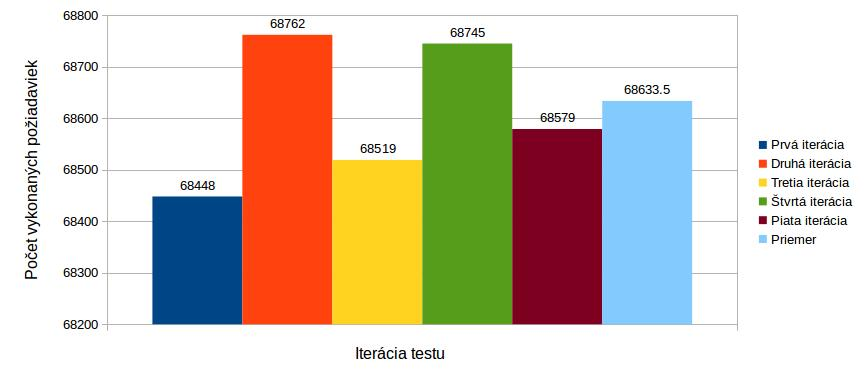
\includegraphics[width=0.9\textwidth]{gatling3_3.jpg}
  \caption{Celkový počet vykonaných požiadaviek}
\end{figure}

\begin{figure}[H]
  \centering
      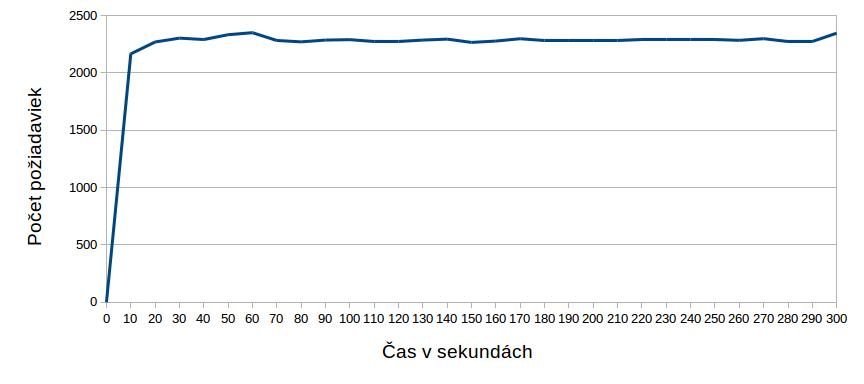
\includegraphics[width=0.9\textwidth]{gatling3_3_distr.jpg}
  \caption{Časový priebeh vykonaných požiadaviek - aritmetický priemer všetkých iterácií}
\end{figure}

\textbf{Štvrtý test - 51200 znaková správa (50 KB)}
\begin{itemize}

\item[\textbf{1. iterácia}]\ \\
Celkový počet vykonaných požiadaviek: 6829\\
Priemerný počet vykonaných požiadaviek za sekundu: 22,763

\item[\textbf{2. iterácia}]\ \\
Celkový počet vykonaných požiadaviek: 6832\\
Priemerný počet vykonaných požiadaviek za sekundu: 22,773

\item[\textbf{3. iterácia}]\ \\
Celkový počet vykonaných požiadaviek: 6818\\
Priemerný počet vykonaných požiadaviek za sekundu: 22,727

\item[\textbf{4. iterácia}]\ \\
Celkový počet vykonaných požiadaviek: 6806\\
Priemerný počet vykonaných požiadaviek za sekundu: 22,687

\item[\textbf{5. iterácia}]\ \\
Celkový počet vykonaných požiadaviek: 6855\\
Priemerný počet vykonaných požiadaviek za sekundu: 22,850

\item[\textbf{Priemer}]\ \\
Celkový počet vykonaných požiadaviek: 6830,5\\
Priemerný počet vykonaných požiadaviek za sekundu: 22,768

\end{itemize}

\begin{figure}[H]
  \centering
      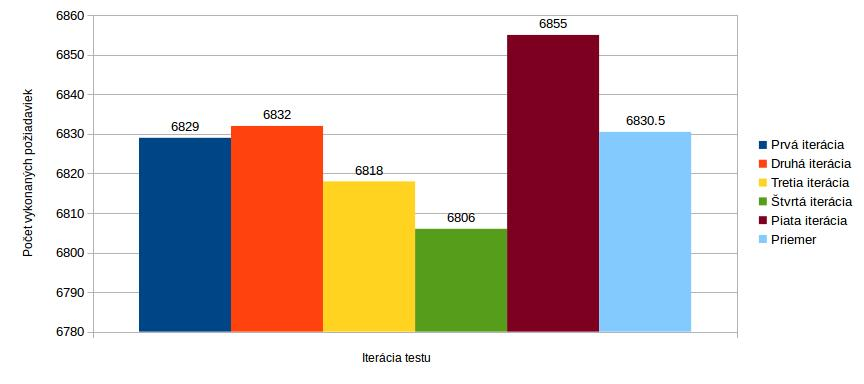
\includegraphics[width=0.9\textwidth]{gatling3_4.jpg}
  \caption{Celkový počet vykonaných požiadaviek}
\end{figure}

\begin{figure}[H]
  \centering
      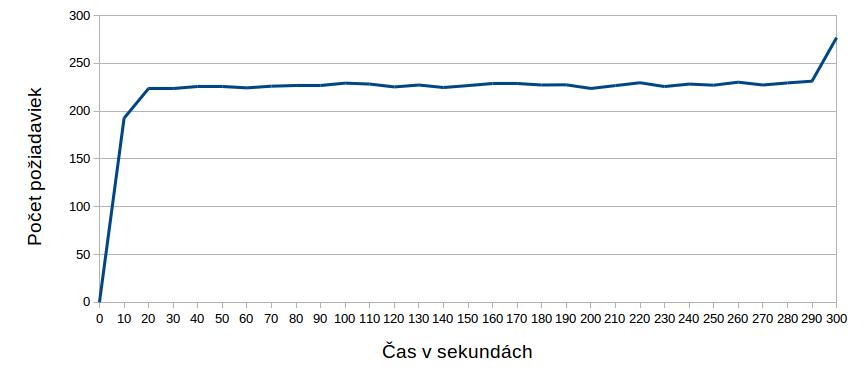
\includegraphics[width=0.9\textwidth]{gatling3_4_distr.jpg}
  \caption{Časový priebeh vykonaných požiadaviek - aritmetický priemer všetkých iterácií}
\end{figure}

\textbf{Piaty test - 512000 znaková správa (500 KB)}
\begin{itemize}

\item[\textbf{1. iterácia}]\ \\
Celkový počet vykonaných požiadaviek: 692\\
Priemerný počet vykonaných požiadaviek za sekundu: 2,307

\item[\textbf{2. iterácia}]\ \\
Celkový počet vykonaných požiadaviek: 692\\
Priemerný počet vykonaných požiadaviek za sekundu: 2,307

\item[\textbf{3. iterácia}]\ \\
Celkový počet vykonaných požiadaviek: 689\\
Priemerný počet vykonaných požiadaviek za sekundu: 2,297

\item[\textbf{4. iterácia}]\ \\
Celkový počet vykonaných požiadaviek: 693\\
Priemerný počet vykonaných požiadaviek za sekundu: 2,310

\item[\textbf{5. iterácia}]\ \\
Celkový počet vykonaných požiadaviek: 689\\
Priemerný počet vykonaných požiadaviek za sekundu: 2,297

\item[\textbf{Priemer}]\ \\
Celkový počet vykonaných požiadaviek: 691,5\\
Priemerný počet vykonaných požiadaviek za sekundu: 2,305

\end{itemize}

\begin{figure}[H]
  \centering
      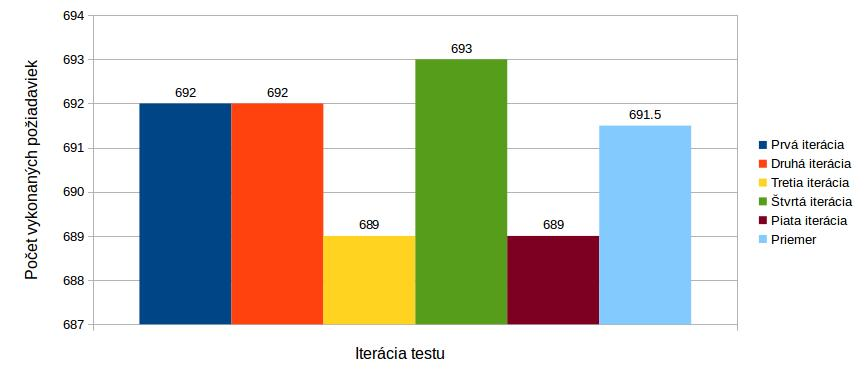
\includegraphics[width=0.9\textwidth]{gatling3_5.jpg}
  \caption{Celkový počet vykonaných požiadaviek}
\end{figure}

\begin{figure}[H]
  \centering
      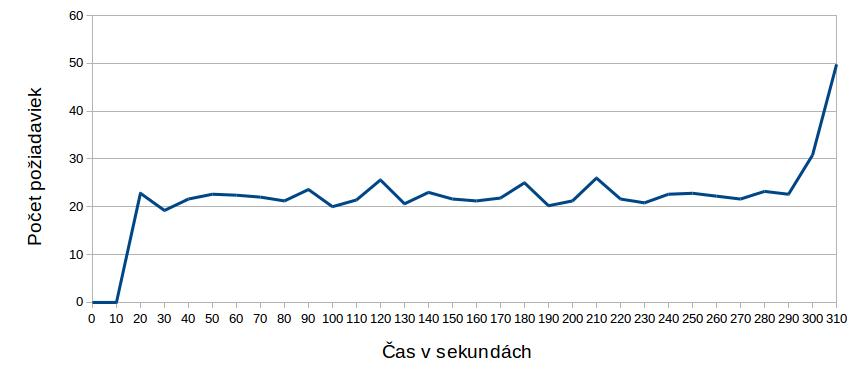
\includegraphics[width=0.9\textwidth]{gatling3_5_distr.jpg}
  \caption{Časový priebeh vykonaných požiadaviek - aritmetický priemer všetkých iterácií}
\end{figure}



\item Perfcake

\end{itemize}

\subsection{Základný JMS test so 100 klientmi}

\begin{itemize}

\item Apache JMeter

\item Faban

Dokumentácia Fabanu neobsahovala žiadne informácie o testovaní JMS. S vynaložením nemalého úsilia sa mi podarilo nájsť na internete blog, ktorý popisoval nastavenie Fabanu, tak aby s ním bolo možné testovať JMS. Článok neobsahoval informácie o nastavení atribútov potrebných pre testovanie JMS. Nadpis článku naznačoval, že existuje pokračovanie, ktoré sa mi nepodarilo nájsť. Z toho usudzujem, že Faban nepodporuje testovanie JMS. Článok bol publikovaný 21.4.2009\cite{FabanBlog}.

\item Gatling

Gatling dokumentácia obsahuje nastavenie testovacieho scenára pre testovanie JMS. Po nastavení všetkých parametrov testu sa pri testovaní objavuje výnimka "{}User NULL"{} naznačujúca, že nie je možné identifikovať užívateľa, pomocou ktorého je možné pristupovať k JMS frontám JBoss AS servera. Meno a heslo užívateľa som nastavil v súlade s návodom a tieto údaje sú rovnaké, ako pri nástrojoch Apache JMeter a Perfcake, u ktorých testy fungujú. Návod je k dispozícii na stránke \url{http://gatling.io/docs/2.1.1/jms.html}.

\item Perfcake

Všetých päť iterácií JMS testu prebehlo bez problémov. Rozptyl medzi maximom a minimom je 2900 vykonaných požiadaviek.

\begin{itemize}

\item[\textbf{1. iterácia}]\ \\
Celkový počet vykonaných požiadaviek: 113714\\
Priemerný počet vykonaných požiadaviek za sekundu: 394.867

\item[\textbf{2. iterácia}]\ \\
Celkový počet vykonaných požiadaviek: 112162\\
Priemerný počet vykonaných požiadaviek za sekundu: 413.784

\item[\textbf{3. iterácia}]\ \\
Celkový počet vykonaných požiadaviek: 112527\\
Priemerný počet vykonaných požiadaviek za sekundu: 388.142

\item[\textbf{4. iterácia}]\ \\
Celkový počet vykonaných požiadaviek: 115062\\
Priemerný počet vykonaných požiadaviek za sekundu: 397.234

\item[\textbf{5. iterácia}]\ \\
Celkový počet vykonaných požiadaviek: 115012\\
Priemerný počet vykonaných požiadaviek za sekundu: 377.893

\item[\textbf{Priemer}]\ \\
Celkový počet vykonaných požiadaviek: 113695.4\\
Priemerný počet vykonaných požiadaviek za sekundu: 378,985	

\end{itemize}

\begin{figure}[H]
  \centering
      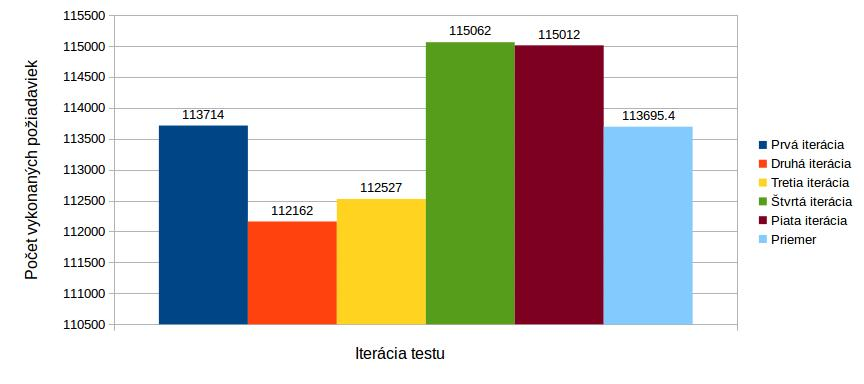
\includegraphics[width=0.9\textwidth]{perfcake4.jpg}
  \caption{Celkový počet vykonaných požiadaviek}
\end{figure}

\begin{figure}[H]
  \centering
      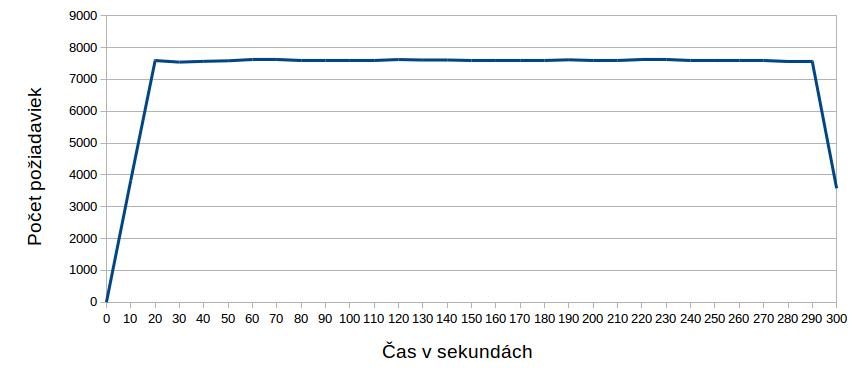
\includegraphics[width=0.9\textwidth]{perfcake4_distr.jpg}
  \caption{Časový priebeh vykonaných požiadaviek - aritmetický priemer všetkých iterácií}
\end{figure}

\end{itemize}

\subsection{Základný test so 100 klientmi}

\begin{itemize}

\item Apache JMeter

\item Faban

\begin{itemize}

\item[\textbf{1. iterácia}]\ \\
Celkový počet vykonaných požiadaviek: 68286\\
Priemerný počet vykonaných požiadaviek za sekundu: 227,620

\item[\textbf{2. iterácia}]\ \\
Celkový počet vykonaných požiadaviek: 68590\\
Priemerný počet vykonaných požiadaviek za sekundu: 228,633

\item[\textbf{3. iterácia}]\ \\
Chyba, \hyperlink{label}{viď. test 2.3.5}.

\item[\textbf{4. iterácia}]\ \\
Celkový počet vykonaných požiadaviek: 67874\\
Priemerný počet vykonaných požiadaviek za sekundu: 226,247

\item[\textbf{5. iterácia}]\ \\
Celkový počet vykonaných požiadaviek: 68567\\
Priemerný počet vykonaných požiadaviek za sekundu: 228,557

\item[\textbf{Priemer}]\ \\
Celkový počet vykonaných požiadaviek: 68329,25\\
Priemerný počet vykonaných požiadaviek za sekundu: 227,764

\end{itemize}

\begin{figure}[H]
  \centering
      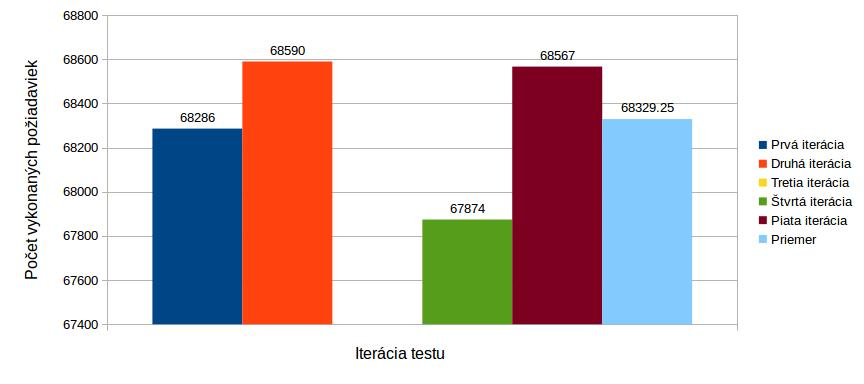
\includegraphics[width=0.9\textwidth]{faban5.jpg}
  \caption{Celkový počet vykonaných požiadaviek}
\end{figure}

\begin{figure}[H]
  \centering
      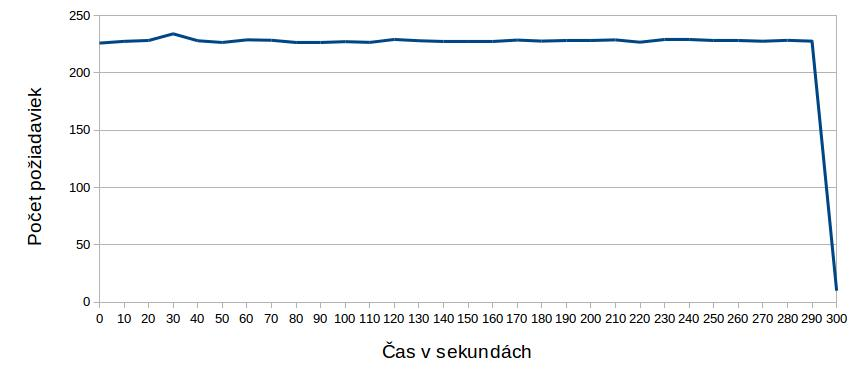
\includegraphics[width=0.9\textwidth]{faban5_distr.jpg}
  \caption{Časový priebeh vykonaných požiadaviek - aritmetický priemer všetkých iterácií}
\end{figure}



\item Gatling

\begin{itemize}

\item[\textbf{1. iterácia}]\ \\
Celkový počet vykonaných požiadaviek: 68775\\
Priemerný počet vykonaných požiadaviek za sekundu: 229,250

\item[\textbf{2. iterácia}]\ \\
Celkový počet vykonaných požiadaviek: 68452\\
Priemerný počet vykonaných požiadaviek za sekundu: 228,173

\item[\textbf{3. iterácia}]\ \\
Celkový počet vykonaných požiadaviek: 68495\\
Priemerný počet vykonaných požiadaviek za sekundu: 228,317

\item[\textbf{4. iterácia}]\ \\
Celkový počet vykonaných požiadaviek: 68273\\
Priemerný počet vykonaných požiadaviek za sekundu: 227,577

\item[\textbf{5. iterácia}]\ \\
Celkový počet vykonaných požiadaviek: 68805\\
Priemerný počet vykonaných požiadaviek za sekundu: 229,350

\item[\textbf{Priemer}]\ \\
Celkový počet vykonaných požiadaviek: 68560\\
Priemerný počet vykonaných požiadaviek za sekundu: 228,533

\end{itemize}

\begin{figure}[H]
  \centering
      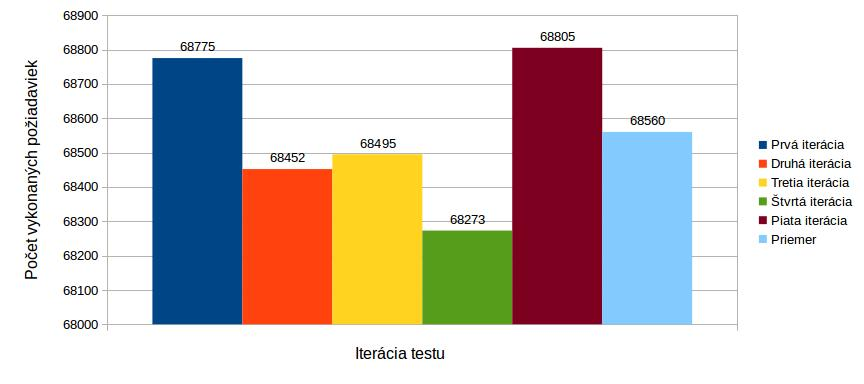
\includegraphics[width=0.9\textwidth]{gatling5.jpg}
  \caption{Celkový počet vykonaných požiadaviek}
\end{figure}

\begin{figure}[H]
  \centering
      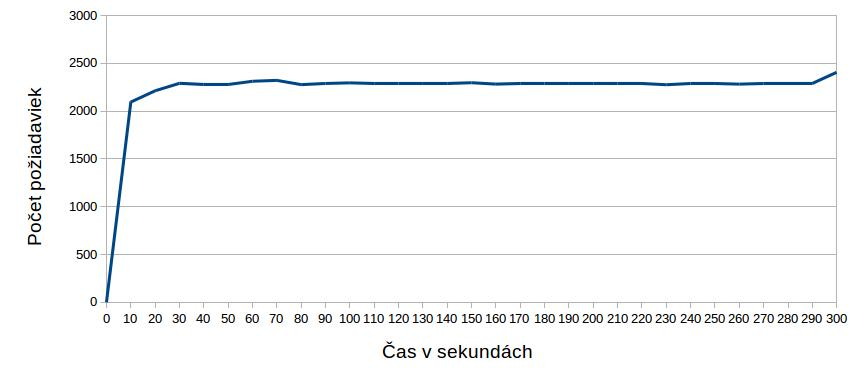
\includegraphics[width=0.9\textwidth]{gatling5_distr.jpg}
  \caption{Časový priebeh vykonaných požiadaviek - aritmetický priemer všetkých iterácií}
\end{figure}


\item Perfcake

\end{itemize}

\subsection{Vytrvalostný test}

\begin{itemize}

\item Apache JMeter

\item Faban

\textbf{Bez úniku pamäte}
\begin{itemize}

\item[\textbf{1. iterácia}]\ \\
Celkový počet vykonaných požiadaviek: 818265\\
Priemerný počet vykonaných požiadaviek za sekundu: 227,296

\item[\textbf{2. iterácia}]\ \\
Celkový počet vykonaných požiadaviek: 823862\\
Priemerný počet vykonaných požiadaviek za sekundu: 228,851

\item[\textbf{3. iterácia}]\ \\
Celkový počet vykonaných požiadaviek: 818863\\
Priemerný počet vykonaných požiadaviek za sekundu: 227,462

\item[\textbf{Priemer}]\ \\
Celkový počet vykonaných požiadaviek: 820330\\
Priemerný počet vykonaných požiadaviek za sekundu: 227,869

\end{itemize}

\begin{figure}[H]
  \centering
      \includegraphics[width=0.9\textwidth]{faban6_no_leak.jpg}
  \caption{Celkový počet vykonaných požiadaviek}
\end{figure}

\textbf{S únikom pamäte}
\begin{itemize}

\item[\textbf{1. iterácia}]\ \\
Celkový počet vykonaných požiadaviek: 822346\\
Priemerný počet vykonaných požiadaviek za sekundu: 228,429

\item[\textbf{2. iterácia}]\ \\
Celkový počet vykonaných požiadaviek: 817627\\
Priemerný počet vykonaných požiadaviek za sekundu: 227,119

\item[\textbf{3. iterácia}]\ \\
Celkový počet vykonaných požiadaviek: 818486\\
Priemerný počet vykonaných požiadaviek za sekundu: 227,357

\item[\textbf{Priemer}]\ \\
Celkový počet vykonaných požiadaviek: 819486,3\\
Priemerný počet vykonaných požiadaviek za sekundu: 227,635

\end{itemize}

\begin{figure}[H]
  \centering
      \includegraphics[width=0.9\textwidth]{faban6_leak.jpg}
  \caption{Celkový počet vykonaných požiadaviek}
\end{figure}

\item Gatling

\item Perfcake

\end{itemize}

\subsection{Test teoretickej priepustnosti nástroja}

\begin{itemize}

\item Apache JMeter

\item Faban

\begin{itemize}

\item[\textbf{1. iterácia}]\ \\
Celkový počet vykonaných požiadaviek: 8385444\\
Priemerný počet vykonaných požiadaviek za sekundu: 27951,480

\item[\textbf{2. iterácia}]\ \\
Celkový počet vykonaných požiadaviek: 8670415\\
Priemerný počet vykonaných požiadaviek za sekundu: 28901,383

\item[\textbf{3. iterácia}]\ \\
Celkový počet vykonaných požiadaviek: 8810458\\
Priemerný počet vykonaných požiadaviek za sekundu: 29368,193

\item[\textbf{4. iterácia}]\ \\
Celkový počet vykonaných požiadaviek: 8775981\\
Priemerný počet vykonaných požiadaviek za sekundu: 29253,270

\item[\textbf{5. iterácia}]\ \\
Celkový počet vykonaných požiadaviek: 8762981\\
Priemerný počet vykonaných požiadaviek za sekundu: 29209,937

\item[\textbf{Priemer}]\ \\
Celkový počet vykonaných požiadaviek: 8681055,8\\
Priemerný počet vykonaných požiadaviek za sekundu: 28936,853

\end{itemize}

\begin{figure}[H]
  \centering
      \includegraphics[width=0.9\textwidth]{faban7.jpg}
  \caption{Celkový počet vykonaných požiadaviek}
\end{figure}

\begin{figure}[H]
  \centering
      \includegraphics[width=0.9\textwidth]{faban7_distr.jpg}
  \caption{Časový priebeh vykonaných požiadaviek - aritmetický priemer všetkých iterácií}
\end{figure}



\item Gatling



\begin{itemize}

\item[\textbf{1. iterácia}]\ \\
Celkový počet vykonaných požiadaviek: 3044179\\
Priemerný počet vykonaných požiadaviek za sekundu: 10147,263

\item[\textbf{2. iterácia}]\ \\
Celkový počet vykonaných požiadaviek: 2846062\\
Priemerný počet vykonaných požiadaviek za sekundu: 9486,873

\item[\textbf{3. iterácia}]\ \\
Celkový počet vykonaných požiadaviek: 2989634\\
Priemerný počet vykonaných požiadaviek za sekundu: 9965,447

\item[\textbf{4. iterácia}]\ \\
Celkový počet vykonaných požiadaviek: 3034939\\
Priemerný počet vykonaných požiadaviek za sekundu: 10116,463

\item[\textbf{5. iterácia}]\ \\
Celkový počet vykonaných požiadaviek: 2979783\\
Priemerný počet vykonaných požiadaviek za sekundu: 9932,610

\item[\textbf{Priemer}]\ \\
Celkový počet vykonaných požiadaviek: 2978919,4\\
Priemerný počet vykonaných požiadaviek za sekundu: 9929,731

\end{itemize}

\begin{figure}[H]
  \centering
      \includegraphics[width=0.9\textwidth]{gatling7.jpg}
  \caption{Celkový počet vykonaných požiadaviek}
\end{figure}

\begin{figure}[H]
  \centering
      \includegraphics[width=0.9\textwidth]{gatling7_distr.jpg}
  \caption{Časový priebeh vykonaných požiadaviek - aritmetický priemer všetkých iterácií}
\end{figure}


\item Perfcake

\end{itemize}


\chapter{Záver}


\section{Zhrnutie}

\textbf{Apache Jmeter}
\newline \\
Plusy
\begin{itemize}
\item[+] Podpora pre IDE
\item[+] Wiki a FAQ stránky
\item[+] Je súčasťou ubuntu softvérového centra \\
\end{itemize}

\noindent Mínusy
\begin{itemize}
\item[-] Chýbajúce informácie o ďalšom vývoji
\item[-] Miestami zastaralá dokumentácia \\
\end{itemize}

\noindent \textbf{Perfcake}
\newline \\
Plusy
\begin{itemize}
\item[+] Aktívny vývoj nových verzií
\item[+] Prehľadná dokumentácia
\item[+] Strmá krivka učenia \\
\end{itemize}

\newpage

\noindent Mínusy
\begin{itemize}
\item[-] Neexistuje grafické prostredie
\item[-] Potrebná základná znalosť značkovacých jazykov \\
\end{itemize}

\noindent \textbf{Faban}
\newline \\
Plusy
\begin{itemize}
\item[+] SPECS
\end{itemize}

\noindent Mínusy
\begin{itemize}
\item[-] Chýbajúca podpora pre IDE
\item[-] Neaktívny vývoj
\item[-] Port 9999 používa Faban, aj JBoss AS
\item[-] Najaktuálnejšia verzia bola vydaná 26.9.2013 
\item[-] Zložitá tvorba a upravovanie scenárov \\
\end{itemize}


\noindent \textbf{Gatling}
\newline \\
Plusy
\begin{itemize}
\item[+] Dokumentácia
\item[+] Výsledky zobrazené v grafickom prostredí
\end{itemize}

\noindent Mínusy
\begin{itemize}
\item[-] Chýbajúce informácie o ďalšom vývoji
\item[-] Úprava a tvorba scenárov vyžaduje znalosti jazyka Scala
\item[-] Neexistuje grafické prostredie \\
\end{itemize}

\bibliographystyle{unsrt}
\bibliography{bibliography}

\appendix
\chapter{Obsah priloženého CD}
Súčasťou tejto práce je aj CD obsahujúce všetky materiály, ktoré boli vytvorené v rámci písania práce. Adresárová štruktúra CD vyzerá nasledovne:

\bigskip

\dirtree{%
.1 /.
.2 Bakalárska práca.
.3 img\DTcomment{Adresár s obrázkami použitými v práci}.
.3 bibliografie.bib\DTcomment{Bibliografická databáza práce}.
.3 bp.tex\DTcomment{Zdrojový kód práce}.
.3 bp.pdf\DTcomment{Hotová práca}.
.2 klient.zip\DTcomment{Archív obsahujúci klientskú časť testov}.
.3 1, 2, 3, 4, 5, 6, 7\DTcomment{Symbolické odkazy k adresárom}.
.3 1.Zakladny\ test\ s\ jednym\ klientom\DTcomment{Adresár s testom}.
.3 2.Rastuce\ mnozstvo\ klientov\DTcomment{Adresár s testom}.
.3 3.Rastuca\ velkost\ spravy\DTcomment{Adresár s testom}.
.3 4.JMS zakladny test so 100 klientmi\DTcomment{Adresár s testom}.
.3 5.Zakladny\ test\ so 100 klientmi\DTcomment{Adresár s testom}.
.3 6.Vytrvalostny\ test\DTcomment{Adresár s testom}.
.3 7.Test\ teoretickej priepustnosti nastrojov\DTcomment{Adresár s testom}.
.3 Nastroje\DTcomment{Adresár obsahujúci nástroje}.
.4 apache-jmeter-2.11\DTcomment{Nástroj Apache JMeter}.
.4 faban\DTcomment{Nástroj Faban}.
.4 gatling-charts-highcharts-2.0.1\DTcomment{Nástroj Gatling}.
.4 change\underscore{}runtime.sh\DTcomment{Skript meniaci čas testov}.
.4 change\underscore{}server\underscore{}and\underscore{}port.sh\DTcomment{Skript meniaci server a port}.
.4 open\underscore{}scenarios.sh\DTcomment{Skript otvárajúci scenáre}.
.4 remove\underscore{}all\underscore{}logs.sh\DTcomment{Skript odstraňujúci všetky logy a reporty}.
.4 remove\underscore{}big\underscore{}logs.sh\DTcomment{Skript odstraňujúci velké logy a reporty}.
.4 restart\underscore{}faban.sh\DTcomment{Skript reštartujúci Faban server}.
.4 run\underscore{}all.sh\DTcomment{Skript spúšťajúci testy}.
.2 server.zip\DTcomment{Archív obsahujúci serverovú časť testov}.
.3 Nastroje\DTcomment{Adresár obsahujúci JBoss AS server}.
.4 jboss-as-7.1.1.Final\DTcomment{JBoss AS server}.
.3 ssh\underscore{}restart\underscore{}jboss.sh\DTcomment{Skript reštartujúci JBoss AS server}.
}

\bigskip

\end{document}
